%%%%%%%%%%%%%%%%%%%%%%%%%%%%%%%%%%%%%%%%%%%%%%%%%%%%%%%%%%%%
% This is the official template for theses and seminar papers from the Chair for Information Systems for Sustainable Society (IS3) at the University of Cologne

%
%PREAMBLE
%%%%%%%%%%%%%%%%%%%%%%%%%%%%%%%%%%%%%%%%%%%%%%%%%%%%%%%%%%%%%

\documentclass[a4paper, twoside, 12pt]{article}
\usepackage[utf8]{inputenc}
\usepackage[spanish]{babel}
\usepackage[T1]{fontenc}
\usepackage{graphicx}
\usepackage{longtable}
\usepackage{hyperref}
\usepackage{xcolor}
\usepackage{caption}
\usepackage{epigraph}
\usepackage{subcaption}
\usepackage{amssymb}
\usepackage{amsmath}
\usepackage{listings}

\colorlet{mygray}{black!30}
\colorlet{mygreen}{green!60!blue}
\colorlet{mymauve}{red!60!blue}

\lstset{
  backgroundcolor=\color{gray!10},
  basicstyle=\ttfamily,
  columns=fullflexible,
  breakatwhitespace=false,
  breaklines=true,
  captionpos=b,
  commentstyle=\color{mygreen},
  extendedchars=true,
  frame=single,
  keepspaces=true,
  keywordstyle=\color{blue},
  language=c++,
  numbers=none,
  numbersep=5pt,
  numberstyle=\tiny\color{blue},
  rulecolor=\color{mygray},
  showspaces=false,
  showtabs=false,
  stepnumber=5,
  stringstyle=\color{mymauve},
  tabsize=3,
  title=\lstname
}

% set margins for double-sided printing
\usepackage[left=2.5cm, right=2.5cm, top=2.5cm, bottom=2.5cm, bindingoffset=1.5cm, head=15pt]{geometry}
\usepackage{setspace}
\onehalfspacing
% set headers
\usepackage{fancyhdr}
\pagestyle{fancy}
\fancyhead{}
\fancyfoot{}
\fancyhead[LE,RO]{\textsl{\leftmark}}
\fancyhead[RE,LO]{\thesisauthor}
\fancyfoot[C]{\thepage}
\renewcommand{\headrulewidth}{0.4pt}
\renewcommand{\footrulewidth}{0pt}

% set APA citation style
%\usepackage{apacite}
%\usepackage{biblatex}
%\addbibresource{Bibliography.bib}
\usepackage[nottoc]{tocbibind}
\usepackage[square,numbers]{natbib}
\bibliographystyle{dinat}
%\usepackage{biblatex}
\pagenumbering{gobble}

%%%%%%%%%%%%%%%%%%%%%%%%%%%%%%%%%%%%%%%%%%%%%%%%%%%%%%%%%%%%%
%THESIS Parameters
%%%%%%%%%%%%%%%%%%%%%%%%%%%%%%%%%%%%%%%%%%%%%%%%%%%%%%%%%%%%%

\title{Estudio computacional de la dinámica estructural del
ADN, posterior a su interacción con radiación ionizante}

\newcommand{\thesisdate}{January 01, 2019}
\newcommand{\thesisauthor}{Jaiver Estiven Salazar Ortiz} %input name
\newcommand{\thesistype}{Informe Final de Pasantía} % Set either to Bachelor or Master
\newcommand{\supervisor}{Edwin Munévar}
\newcommand{\cosupervisor}{Alfonso Leyva}



%%%%%%%%%%%%%%%%%%%%%%%%%%%%%%%%%%%%%%%%%%%%%%%%%%%%%%%%%%%%%
%DOCUMENT
%%%%%%%%%%%%%%%%%%%%%%%%%%%%%%%%%%%%%%%%%%%%%%%%%%%%%%%%%%%%

\setcounter{tocdepth}{4}
\setcounter{secnumdepth}{4}

\setcounter{tocdepth}{5}
\setcounter{secnumdepth}{5}

\setcounter{tocdepth}{6}
\setcounter{secnumdepth}{6}

\makeatletter
\newcounter{subsubparagraph}[subparagraph]
\renewcommand\thesubsubparagraph{%
  \thesubparagraph.\@arabic\c@subsubparagraph}
\newcommand\subsubparagraph{%
  \@startsection{subsubparagraph}    % counter
    {6}                              % level
    {\parindent}                     % indent
    {3.25ex \@plus 1ex \@minus .2ex} % beforeskip
    {-1em}                           % afterskip
    {\normalfont\normalsize\bfseries}}
\newcommand\l@subsubparagraph{\@dottedtocline{6}{13em}{5em}}
\newcommand{\subsubparagraphmark}[1]{}
\makeatother

\begin{document}

%%%%%%%%%%%%%%%%%%%%%%%%%%%%%%%%%%%%%%%%%%%%%%%%%%%%%%%%%%%%%
%TITLE PAGE (Pre-defined, just change parameters above)
%%%%%%%%%%%%%%%%%%%%%%%%%%%%%%%%%%%%%%%%%%%%%%%%%%%%%%%%%%%%%
%%%%%%%%%%%%%%%%%%%%%%%%%%%%%%%%%%%%%%%%%%%%%%%%%%%%%%%%%%%%%
%TITLE PAGE
%%%%%%%%%%%%%%%%%%%%%%%%%%%%%%%%%%%%%%%%%%%%%%%%%%%%%%%%%%%%%
\makeatletter
\begin{titlepage}
    \begin{center}
        \vspace*{1cm}

        \Large
        \textbf{\@title}

        \vspace{1.5cm}
        
        \thesistype{}
        
        \vspace{1cm}

        \begin{figure}[htbp]
             \centering
             
\includegraphics[width=.5\linewidth]{./Figures/UoC_Logo.png}
        \end{figure}

        \vspace{1cm}

        \large
        \textbf{Autor}: \thesisauthor{}\\
        \large
        \textbf{Supervisor}: \supervisor{}\\
        \large
        \textbf{Co-Supervisor}: \cosupervisor{}

        \vspace{1cm}
        \large
        Proyecto Curricular de Licenciatura en Física\\
        Facultad de Ciencias y Educación\\
        Universidad Distrital Francisco José de Caldas\\

        \vspace{1cm}
        \@date

    \end{center}
\end{titlepage}
\makeatother

%%%%%%%%%%%%%%%%%%%%%%%%%%%%%%%%%%%%%%%%%%%%%%%%%%%%%%%%%%%%%
%SOOA
%%%%%%%%%%%%%%%%%%%%%%%%%%%%%%%%%%%%%%%%%%%%%%%%%%%%%%%%%%%%%
\epigraph{“Now I'm a scientific expert; that means I know nothing about absolutely everything.”}
{― Arthur C. Clarke, 2001: A Space Odyssey}

\clearpage
\thispagestyle{empty}
\section*{Agradecimientos}
\label{sec:SOOA}

\vspace{2.5cm}

% Statement of original authorship - Needs to be in German
% see also here: https://www.wiso.uni-koeln.de/sites/fakultaet/dokumente/PA/formulare/eidesstattliche_erklaerung.pdf

Este trabajo marca una cumbre en mi vida y una transición de la que considero hasta el momento la mejor etapa de la misma hacia un futuro con infinidad de posibilidades debido a lo que he aprendido en estos años, las experiencias tanto buenas como malas con todas las personas que llegue a conocer, junto con todo el apoyo que he recibido el cual sinceramente no siento que merezca.\\

Esto no habría sido posible sin el amor incondicional de mis padres, de mi hermano, y demás familiares.\\

Quiero agradecer especialmente a los Profesores Edwin Munévar y Alfonso Leyva quienes siempre estuvieron para apoyarme y nunca desistieron con mi aprendizaje.\\


A todos ellos: \\
No tengo las palabras suficientes para describir cuanto les debo.

\vspace{1cm}



\vspace{3cm}
\noindent
\textbf{\thesisauthor{}}

\vspace{0.5cm}
\noindent
Bogotá D.C 22.10.2019


%%%%%%%%%%%%%%%%%%%%%%%%%%%%%%%%%%%%%%%%%%%%%%%%%%%%%%%%%%%%%
%ABSTRACT
%%%%%%%%%%%%%%%%%%%%%%%%%%%%%%%%%%%%%%%%%%%%%%%%%%%%%%%%%%%%%
%\clearpage
%\thispagestyle{empty}
%\section*{Abstract}

%[Abstract goes here (max. 1 page)]



%%%%%%%%%%%%%%%%%%%%%%%%%%%%%%%%%%%%%%%%%%%%%%%%%%%%%%%%%%%%%
%TOC,TOF,TOT
%%%%%%%%%%%%%%%%%%%%%%%%%%%%%%%%%%%%%%%%%%%%%%%%%%%%%%%%%%%%%
\clearpage
\pagenumbering{Roman}
\tableofcontents
\clearpage
\listoffigures
\clearpage
%\listoftables
%\clearpage

\pagenumbering{arabic}


%%%%%%%%%%%%%%%%%%%%%%%%%%%%%%%%%%%%%%%%%%%%%%%%%%%%%%%%%%%%%
%MAIN PART
%%%%%%%%%%%%%%%%%%%%%%%%%%%%%%%%%%%%%%%%%%%%%%%%%%%%%%%%%%%%%

%\input{./Sections/Seccion0}

% SEC1
\clearpage
\section{Consideraciones}

\subsection{Justificación}
\label{sec:Intro}
El siguiente trabajo fue llevado acabo en la Pontificia Universidad Javeriana en Bogotá D.C en colaboración con los profesores Edwin Munevar y Alfonso Leyva. En si el estudio del ADN es fundamental hoy día, y abarca un sin fin de incógnitas que de llegar a resolverse pueden aportar significativamente a tratar diversas enfermedades entre las cuales se encuentra el cáncer, este trabajo se basa en la interacción del ADN con la radiación y de su estudio con herramientas computacionales con el fin de entender un poco más de como son las interacciones y los diversos fenómenos que acompañan esto.
\subsection{Objetivos}
\subsubsection{Objetivo General}
\begin{itemize}
  \item Estudiar el efecto de la radiación ionizante sobre los enlaces químicos que definen la estructura tridimensional de una macromolécula de ADN.
\end{itemize}
\subsubsection{Objetivos Específicos}
\begin{itemize}
  \item A partir de un código base “Geant4-DNA” estructurar un programa que permita realizar apropiadamente la simulación del ADN y su interacción con radiación ionizante.
  \item Basados en los resultados de la simulación se determina los efectos de la radiación sobre la estructura misma de la bio-macromolécula
  \item Mediante el análisis de los resultados obtenidos, tener la debida dinámica propia de la bio-macromolécula luego de haber sido irradiada.
\end{itemize}
\subsubsection{Resultados alcanzados}
En base al proyecto de grado junto con su debido cronograma de actividades se obtuvieron los siguientes resultados:
\begin{itemize}
  \item Se construyo un referente bibliográfico
a partir de diferentes fuentes de información tales como
artículos, libros y manuales, con el fin de establecer los conceptos necesarios y tener la información adecuada.
\item Se realizo el debido entrenamiento del software, entre lo que se encuentra el uso de ROOT para generar histogramas, VMD( visual molecular dinamics) un software desarrollado por la universidad Illinois para la visualización de moléculas, GEANT4 toolkit para el estudio de partículas cargadas a través de la materia y por ultimo gromacs un sotfware encargado de la simulación de la dinámica molecular de sistemas en los que se encuentran proteínas, lipidos y ácidos nucleicos.
\item Se estudio y se modifico un ejemplo muy especifico y complejo de Geant4 conocido como pdb4dna, de este se obtuvieron diversos resultados para el análisis de una macromolécula de ADN.
\end{itemize}


% SEC2

\clearpage

\section{Una revisión al ADN}
\label{sec:Intro}
La importancia de este capitulo es dar las bases necesarias para ADN


\subsection{Historia del ADN}
La epopeya del ADN tiene sus inicios en 1869 con un bioquímico llamado Friedrich Miescher, esté estaba interesado en la estructura química de las fascinantes unidades fundamentales de la vida conocidas como células.
Miescher viajaba todos los días a la clínica más cercana para tomar las vendas sucias, esto debido a que estaban recubiertas de pus (lo cual era una buena fuente de leucocitos), añadiendo álcali hizo que los núcleos se abrieran liberando sus componentes, de esta manera Miescher extrajo un componente(ADN), al que el nombro nucleína, realizando un análisis de esta nucleína mostró que era un ácido que contenía fósforo y por tanto no calificaba en en ninguno de los grupos conocidos en ese momento como carbohidratos y proteínas, este fue clasificado como un ácido nucleico y su relevancia biológica no fue descubierta hasta mucho tiempo después \cite{Susan}.\\

En 1928 Fredrick Griffith realizaba una investigación con neumococos, tenia dos tipos: el primero patógeno  fue cultivado en placas de petri conocido como s(smooth-suave) debido a su apariencia, el segundo inofensivo y conocido como r(rough-áspero), Griffith descubrio que al añadir un extracto de los neumococos tipos S al tipo R, esté ultimo podría heredar las propiedades del tipo S, este -principio de transformación- indicaba que el extracto contenía la molécula de herencia.\\

Oswald Avery junto con MacLeod y McCarty demostrarón que substancia efectiva en el experimento de Griffiths era la molecula de ADN y que a su vez, era el portador de genes en la célula, también es importante mencionar que Alfred Hershey y Martha Chase quienes confirmaron la conclusión en 1952 mediante experimentos con trazadores radioactivos\cite{Thormod}.\\

Es relevante mencionar otros aportes significativos: \\
1.Erwin Chargaff encontro una regularidad peculiar en los radios de las bases de los nucleotidos.\\
2.Sven Furger trabajo en la estructura de los componentes del ADN, encontró que la base plana(plano de la citocina) era perpendicular a la molecula de azucar.\\
3.Rosalind Franklin logro distinguir dos tipos de ADN dependiendo de la hidratación y que ambos tenían estructura helicoidal mediante cristalográfia, véase figura ~\ref{fig:rf}.

\begin{figure}[htbp]
    \centering
    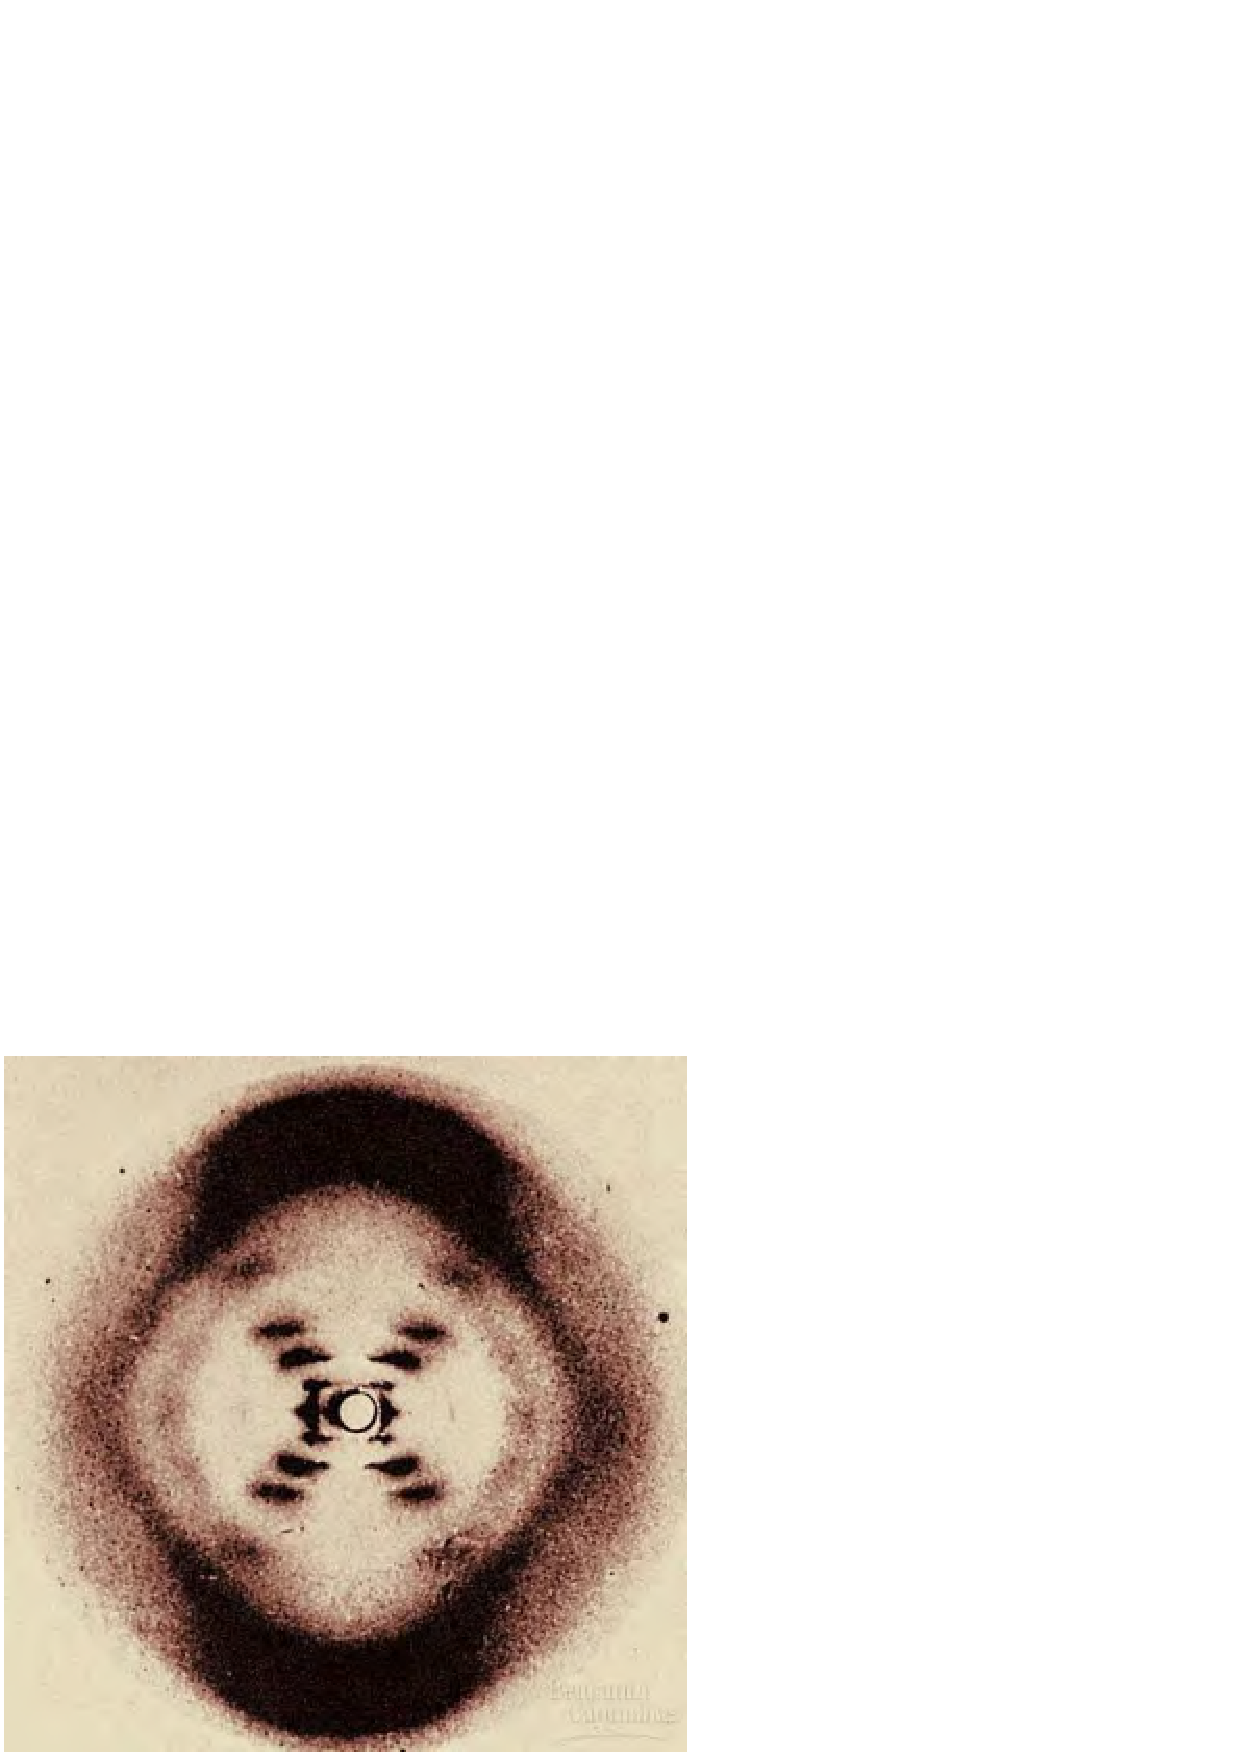
\includegraphics[width=0.5\linewidth]{./Figures/RF.png}
    \caption[Fotografía cristalográfica del ADN]{Fotografiá cristalográfica del ADN tomada por Rosalind Franklin en 1952}
    \label{fig:rf}
\end{figure}
El ultimo paso hacia la estructura del ADN fue llevado acabo por James Watson y Francis Crick en el laboratorio de Cavendish en francia, juntos trabajarón en diferentes modelos de la molecula de ADN , en 1953 publicarón un articulo en la prestigiosa revista Nature titulado: "Molecular Structure of Nucleid Acids", el articulo solo tenia una pagina, pero era de un impacto significativo debido al modelo de ADN que contenía, un modelo de doble hélice(figura ~\ref{fig:jw}), y sugerían que el emparejamiento  especifico que habían postulado intuía un posible mecanismo para copiar material genético.
\begin{figure}[htbp]
    \centering
    
\includegraphics[width=0.15\linewidth]{./Figures/DNA1.png}
    \caption[Diagrama esquemático del ADN]{Diagrama esquemático del ADN publicado por Watson y Crick en 1953, imagen tomada de \cite{jwfc}.}
    \label{fig:jw}
\end{figure}
\subsection{Estructura del ADN}
El ADN es una molécula compuesta por seis diferentes tipos de bloques: cuatro bases, citocina, timina, guanina, adenina, junto con una molécula de azúcar y un grupo fosfato, el fosfato el azucar y la base forman un nucleotido, y el ADN esta conformado por dos cadenas largas de nucleotidos
If all the DNA in a single human cell was tied together and stretched out, it would be approximately 2 meters long. One strand of DNA binds to the other strand through hydrogen bonds that extend between base pairs. Thus, C binds specifically with G and A binds with T forming the C – G and A – T base pairs.
The human double helix contains about 6 billion base pairs. Three adjacent bases (a triplet or codon) on one strand code for a certain amino acid in a protein. If a protein consists of 200 amino acids, the DNA that codes for this protein consists of at least 600 bases, i.e., 200 triplet codons. This is a gene.

\subsubsection{Daño inducido por radiación al ADN}
The most important types of damage to the DNA molecule, induced by radiation, are outlined in the figure below. There are four common types of damage
\paragraph{Rompimientos simples}
A single strand break is simply a break in one of the sugar-phosphate chains. This damage is usually simple to repair and, in experiments, it has been shown that approximately 90\% of the single strand breaks are repaired in the course of one hour at 37o
C. 2.
\paragraph{Rompimientos dobles}
This type of damage involves both strands of the DNA helix, which are broken opposite to each other or within a distance of a few base pairs. This type of damage (also called a clustered damage) would kill the cell and in experiments with bacteria a correlation is found between double strand breaks and cell death (David Freifelder in the 1960-ties).
Double strand breaks are more difficult to repair correctly. However, they actually are. The DNA-molecule is packed together with proteins supporting the structure and preventing the pieces from falling apart, even when breaks occur on both strands of the helix. There are in fact a number of mechanisms that complex organisms (such as humans) have evolved for repairing double strand breaks. But as one might guess, this type of break is more difficult to repair and does correlate with cell death and observable damage to chromosomes.
3.
\paragraph{Daño base}
Experiments indicate that the radiation sensitivity varies from one base to another. After an initial ionization, rapid electronic reorganizations take place with the result that the damage is transported to certain regions of the macromolecule. The base guanine is particularly sensitive.
Damage to a base is one of the starting points for a mutation. If a base is changed, information may be lost or changed. As the result of a misrepair or no repair, the altered triplet codon is likely to lead to insertion of the incorrect amino acid in the pro- tein. In turn, the changed protein might not function properly.
\paragraph{Dimeridos de pirimidina}
Pyrimidine dimers are also examples of clustered damage. In this example, two adjacent bases, T and T, on the same strand have been chemically altered.
This is but one out of a
myriad of possibilities. All the possibilities have the common feature that two or more damaged sites lie in close proximity to one another.
Double strand break
Base damage
We shall return to repair mechanisms, but would like to mention the problems posed by clustered damage. One of the strands is needed to replicate the adjacent strand. When both strands are damaged at the same site there is no template to work from. This is in contrast to damage such as a single base alteration or a single strand break
\subsection{Daño Celular}
\subsubsection{Reparación del ADN}
\subsubsection{Mecanismos de defensa}
\subsubsection{Respuesta adaptativa}


% SEC3

\clearpage

\section{Interacción radiación-materia}
\label{sec:INT}
En general este apartado se basa en dar una pequeña explicación de algunos fenómenos físicos relevantes en la interacción radiación materia, estos se basan en las diversas interacciones de partículas cargadas o fotones con átomos, existen otros procesos que son relevantes como la interacción de neutrones pero debido a que poco tienen que ver(por ahora) con el desarrollo de este trabajo no son incluidos.
\subsection{Interacciones de fotones en la materia}
 A menudo se asume que son solo cuatro los eventos relevantes para fotones al interactuar con átomos: dispersión de Compton, dispersión de Rayleigh, efecto fotoeléctrico, y producción de pares.
Pero en Realidad las interacciones más importantes de fotones con la materia son principalmente seis, las cuales son: dispersión de Compton, dispersión de Rayleigh, efecto fotoeléctrico, producción de nuclear de pares, producción electrónica de pares, y reacciones fotonucleares, esto es debido a que usualmente la producción de nuclear de pares junto a la producción electrónica de pares se manejan ambas bajo el nombre de producción de pares y los efectos de las reacciones fotonucleares son ignorados. A continuación se muestra una explicación sencilla de cada uno de ellos.

\subsubsection{Dispersión de Compton(Dispersión incoherente)}

El efecto Compton recibe su nombre en honor a Arthur Compton quien en 1922 fue la primer persona en realizar mediciones de una dispersión entre un fotón y un electrón libre, este fenómeno se basa en la interacción de un fotón con una energía $h\nu$ junto con un electrón débilmente ligado a un orbital de cierto átomo, cuando esto ocurre, se produce un fotón de energía menor $h\nu '$ y un electrón conocido como el electrón de Compton(dispersado) es expulsado del átomo con una energía cinética $E_k$, es pertinente mencionar que en estudios teóricos se asume que el electrón esta libre y estacionario\cite{Podgorsak}, generalmente es posible usar los cálculos de mecánica clásica con la conservación de energía y momento, sin embargo es importante entender la naturaleza cuántica del proceso, y en particular la transferencia de energía y la asignación de momento a un fotón implicada, los cálculos clásicos funcionan mientras, la velocidad no sea relativista, la energía de los fotones implicados no sea muy baja o el material tenga un numero atómico $Z$ muy alto, si alguna de estas situaciones se cumple es necesario realizar las correcciones apropiadas\cite{Edward}.\\
\begin{figure}[htbp]
    \centering
    \includegraphics[width=.68\linewidth]{./Figures/compton1.eps}
    \caption[Efecto Compton]{Efecto Compton: un fotón incidente con energía $h\nu$ colisiona con un electrón débilmente ligado de un átomo produciendo un fotón con energía menor $h\nu '$ con angulo $\theta$ y a su vez es expulsando un electrón de Compton con energía cinética $E_k$ y angulo $\phi$}
    \label{fig:Compton}
\end{figure}

\subsubsection{Dispersión de Rayleigh(Dispersión coherente)}
Recibe el nombre de Rayleigh debido a el físico John W. Rayleigh quien en 1900 desarrollo una teoría para la dispersión de radiación electromagnética debido a átomos, este fenómeno ocurre principalmente con fotones a bajas energías $h\nu$ junto con un receptor que tenga numero atómico $Z$ alto, consiste en que un fotón incidente es dispersado cuando interactuá con alguno de los electrones ligados a un átomo, el átomo absorbe el momento transferido y el fotón es dispersado con un angulo $\phi$ y con una energía relativamente igual a la que tenía antes de la interacción, los ángulos de este fenómeno son relativamente pequeños dado que la energía impartida al átomo no produce ionización o excitación y este vuelve a su estado original después de la interacción\cite{Podgorsak}.
También se conoce como Dispersión coherente debido a que el fotón es dispersado por  la acción combinada de todo el átomo,debido a esto el evento es elástico en el sentido de que el fotón no pierde casi nada de su energía\cite{Frank}.

\begin{figure}[htbp]
    \centering
    \includegraphics[width=.68\linewidth]{./Figures/Ray.eps}
    \caption[Dispersión de Rayleigh]{Dispersión de Rayleigh:un fotón incidente con energía $h\nu$ interactuá con un electrón ligado a un átomo, este fotón es dispersado con un angulo pequeño $\phi$ y una energía $h\nu '$ relativamente igual a $h\nu$ }
    \label{fig:DR}
\end{figure}


\subsubsection{Efecto fotoeléctrico}

Se conoce como efecto fotoeléctrico a la interacción entre un fotón y un electrón orbital fuertemente ligado a un átomo, el fotón incidente con energía $h\nu$ interactúa con el electrón del átomo, entonces es absorbido completamente y el electrón orbital conocido como fotoelectrón es expulsado con energía cinética $E_k=h\nu-E_B(K)$ Donde $E_B(K)$ es la energía de ionización del electrón, la vacante en el orbital es subsecuentemente tomada por con un electrón más alto y la energía de la transición del electrón sera emitida en la formá de un fotón característico(fluorescencia) o como un electrón de Auger.

A diferencia del efecto Compton el cual ocurre cuando un fotón interactuá con un electrón "libre"(débilmente ligado), el efecto fotoeléctrico sucede entre un fotón y un electrón "ligado fuertemente", la diferencia entre estos radica en la magnitud relativa de la energía del fotón $h\nu$ y la energía necesaria para remover un electrón de un átomo(energía de ionización) $E_B$ en vez de un valor absoluto de $h\nu$ o $E_B$, entonces cuando $E_B\ll h\nu$ se dice que el electrón esta débilmente ligado o libre y cuando  $E_B \lesssim h\nu$ se asume que el electrón esta fuertemente ligado\cite{Podgorsak}.


\begin{figure}[htbp]
    \centering
    \includegraphics[width=.68\linewidth]{./Figures/fotoelec.eps}
    \caption[Efecto fotoeléctrico]{Efecto fotoeléctrico: un fotón incidente con energía $h\nu$ interactúa con el electrón del átomo, entonces es absorbido completamente y el electrón orbital conocido como fotoelectrón es expulsado con energía cinética $E_k$}
    \label{fig:FT}
\end{figure}

\subsubsection{Producción de pares}
Si un fotón con una energía mayor  1.02 MeV entra en un receptor, puede interactuar con los átomos de este por un proceso conocido como producción de pares, en este mecanismo de transferencia de energía el fotón al pasar cerca del átomo esta sujeto a efectos de campo fuerte debido al núcleo, y puede desaparecer y reaparecer como un par de electrones positivo y negativo.\cite{Edward}
Debido a que el momento $p_\nu$ antes de la interacción de producción de pares es mucho más grande que el momento total  $p_{pair}$ después de la interacción de producción de pares,  entonces el fotón debe poseer un exceso de momento que no puede ser absorbido por el par electrón-positrón, por tanto, debe ser absorbido por otro ente de colisión, sea el núcleo atómico, o un electrón orbital\cite{Podgorsak}, dada alguna de estas condiciones tenemos:
\paragraph{Producción nuclear de pares}
 Cuando el fotón interactuá con el núcleo atómico, este juega un rol más o menos pasivo, el estado del núcleo dispersado antes y después del evento es el mismo, excepto por un cambió en su energía cinética y momento. Simplemente un fotón se ha convertido en un electrón y un positrón\cite{Edward}.
\begin{figure}[htbp]
    \centering
    \includegraphics[width=.68\linewidth]{./Figures/nuclearpp.eps}
    \caption[Producción nuclear de pares]{Producción nuclear de pares: Un fotón experimenta una producción de pares estándar, electrón--Positrón}
    \label{fig:PN}
\end{figure}
\paragraph{Producción electrónica de pares}
 El fotón incidente interactúa con un electrón orbital, en lugar de con un núcleo atómico, debido a esto el electrón es dispersado, dado que tiene una masa pequeña, tomará una energía cinética significativa y aparecerá como un producto de la interacción. Además, un electrón y un positrón se generan como resultado de la desaparición del fotón incidente \cite{Edward}.
\begin{figure}[htbp]
    \centering
    \includegraphics[width=.68\linewidth]{./Figures/electpp.eps}
    \caption[Producción electrónica de pares]{Producción electrónica de pares: Un fotón experimenta una producción de pares triple, un electrón dispersado--electrón--Positrón}
    \label{fig:PE}
\end{figure}

\paragraph{Reacciones fotonucleares}
 Usualmente este tipo de fenómeno también recibe el nombre de "fotodesintegración" ó "efecto nuclear fotoeléctrico", se basa en la interacción entre un fotón energético y un núcleo causando desintegración nuclear. En la reacción fotonuclear el núcleo absorbe el fotón y el resultado más probable es la emisión de un solo neutrón, aunque es posible que se emitan otras partículas como $\alpha$, rayos $\gamma$,más de un neutrón o fragmentos de fisión, aunque estos eventos son menos probables, un neutrón producido por este fenómeno se conoce como fotoneutrón\cite{Podgorsak}.

 \begin{figure}[htbp]
     \centering
     \includegraphics[width=.68\linewidth]{./Figures/fotoneu.eps}
     \caption[Reacción fotonuclear]{Reacción fotonuclear: Un fotón es absorbido por un núcleo atómico y este produce un fotoneutrón}
     \label{fig:RF}
 \end{figure}


\subsubsection{Interacciones de partículas cargadas en la materia}
A medida que una partícula viaja en un receptor experimenta interacciones de Coulomb con los núcleos y electrones de los átomos de este mismo, estas interacciones pueden ser divididas en tres categorías dependiendo del tamaño clásico del parámetro de impacto $b$ de la trayectoria de la partícula cargada comparado al radio clásico del átomo $a$ con el que la partícula interactuá.
\paragraph{Colisión de radiación($b\ll a$)}
Cuando el parámetro de impacto $b$ de una partícula cargada es mucho más pequeño que el radio $a$ del átomo, la partícula cargada interactuá más que todo con el núcleo y experimenta dispersión elástica o inelástica junto con un posible cambio en la dirección del movimiento. En la mayoría de los casos se presenta dispersión elástica en cuyo caso la partícula es dispersada por el núcleo pero solo sufre una pequeña perdida de su energía cinética, sin embargo un pequeño porcentaje de estas interacciones son inelasticas y pueden resultar en perdida significante de energía para la partícula cargada acompañada por la emisión de fotones de rayos-x, este tipo de interacción se conoce como colisión de bremsstrahlung\cite{Podgorsak}.


\paragraph{Bremsstrahlung}
Bremsstrahlung es un tipo de fotón de rayos-x producido cuando partículas ligeras experimentan interacción radioactiva inelástica con núcleos de átomos de dado receptor, en esta interacción la partícula presenta ralentización
 dando una fracción significante de energía cinética al fotón\cite{Frank}. Las partículas cargadas de interés para la física medica y dosimetría se pueden clasificar en dos categorías:
\begin{enumerate}
  \item Partículas ligeras cargadas: electrones $e-$ y positrones $e+$, ambos pueden producir fotones bremsstrahlung debido a su masa relativamente pequeña\cite{Podgorsak}.
  \item  Partículas pesadas cargadas: protones $p$, deuterones $d$, partículas alfa $\alpha$, iones pesados tales como $Li^+$,$Be^+$,$C+$,$Ne+$, etc. producen una cantidad insignificante de fotones bremsstrahlung\cite{Podgorsak}.
\end{enumerate}


Bremsstrahlung es la palabra en alemán para designar radiación de frenado.

\begin{figure}[htbp]
   \centering
   \includegraphics[width=.6\linewidth]{./Figures/radiacol.eps}
   \caption[Colisión de radiación]{Colisión de radiación(producción de bremsstrahlung)}
   \label{fig:B}
\end{figure}


\paragraph{Colisión fuerte($b\approx a$)}
Cuando el parámetro $b$ de la trayectoria de una partícula cargada sea aproximadamente del orden del radio $a$ del átomo,la partícula cargada puede tener un impacto directo de Coulomb con un electrón de un orbital, a este fenómeno se le conoce como Colisión fuerte en el cual se transfiere una cantidad significante de energía de la partícula al electrón, luego de la interacción el electrón deja el átomo como un rayo $\gamma$, el numero de colisiones fuertes que  experimenta  una partícula cargada moviéndose en un receptor es generalmente pequeño, sin embargo la transferencia de energía asociada es relativamente grande\cite{Podgorsak}.


\begin{figure}[htbp]
   \centering
   \includegraphics[width=.6\linewidth]{./Figures/hardcoli.eps}
   \caption{Colisión fuerte}
   \label{fig:cf}
\end{figure}

\paragraph{Colisión debil($b\gg a$)}
Cando el parámetro $b$ de la partícula cargada es mucho más grande que el radio $a$ del átomo, la partícula cargada interactuá con todo el átomo el cual se compone de electrones ligados, la energía transferida por la partícula cargada en este evento a los electrones ligados es muy pequeña, sin embargo el numero de estas interacciones es bastante grande, y debido a esto la partícula pierde mucha energía, estas mini-interacciones pueden causar polarización atómica, excitación o ionización mediante la remoción de un electrón de valencia, este fenómeno recibe el nombre de colisión débil o colisión suave\cite{Podgorsak}.

\begin{figure}[htbp]
   \centering
   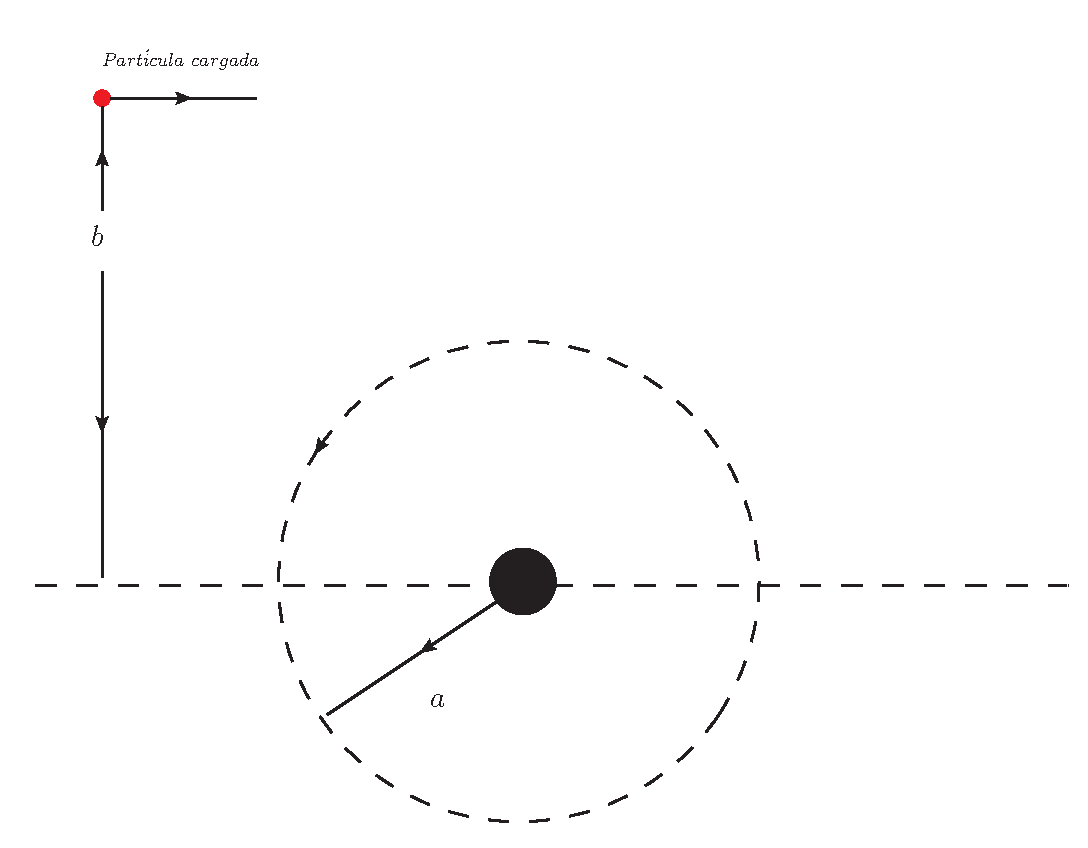
\includegraphics[width=.6\linewidth]{./Figures/softcoli.eps}
   \caption{Colisión débil o suave}
   \label{fig:cd}
\end{figure}


% SEC4

\clearpage

\section{GEANT4}
\label{sec:GEANT4}
GEANT4(\textbf{GE}ometry \textbf{AN}d \textbf{T}racking - \textbf{4} versión) es una plataforma computacional para la simulación de diversos procesos físicos que se centra en la interacción de partículas viajando a través de la materia haciendo uso de monte carlo. Geant es creado en 1974 por el CERN pensado originalmente para la simulación de experimentos en física de altas energías, esto cambiaría con el desarrollo de subsecuentes versiones las cuales serían empleadas en muchos otros campos, su cuarta versión Geant4 es publicada en 1998, esta ultima a su vez también ha tenido diversas versiones actualizadas cada año, su lanzamiento más reciente ha sido Geant4-10.5.p01 y su versión beta Geant4-10.6-beta ambas versiones liberadas en el presente año,  cuenta  con áreas de aplicación que incluyen física de altas energías, física espacial, física médica, transferencia tecnológica, entre otras, su desarrollo, aplicación y mantenimiento son debido al equipo colaborativo a nivel global Geant4 Colaboration los cuales se centran en que el software pueda ser lo mejor posible.
\\
\\
GEANT4 se proporciona bajo la licencia \href{https://geant4.web.cern.ch/license/LICENSE.html}{\color{blue}{Geant4 Software License}}.

\subsection{PDB4DNA}

PPB4DNA es una aplicación relativamente nueva de Geant4 creada por Geant4-DNA project, se basa en el uso adicional de una librería construida en c++ llamada PDBlib, la cual permite hacer uso de la estructura atómica de una molécula de ADN al extraer datos que se encuentran en un archivo .pdb para posteriormente ser usados en Geant4 para evaluar el daño inducido por partículas ionizantes al mismo, mediante un conteo de rompimientos simples, rompimientos dobles y su correspondiente deposición de energía.

El objetivo principal de Geant4-DNA project  es extender Geant4 con diversos procesos para el modelar el daño biológico inducido por radiación ionizante en la escala del ADN, es coordinado desde el 2008 por el National Institute for Nuclear and Particle Physics (IN2P3) del National Centre for Scientific Research (CNRS) en Francia.


\subsubsection{PDB}
Un archivo .pdb (Protein Data Bank) es un archivo de texto que contiene la información estructural de una molécula, se compone de cientos a miles de lineas y en general debe contener lo siguiente\\
HEADER: Registra si la molécula es ADN o proteína.\\
REMARK: Designa comentarios los cuales pueden dar información relevante.\\
ATOM: Registra el símbolo del átomo, id de cadena, numero de residuo o nucleótido y coordenadas espaciales x y z. \\
Para observar un ejemplo de como esta conformado un archivo pdb véase figura ~\ref{fig:pdbesq}.
\begin{figure}[htbp]
    \centering
    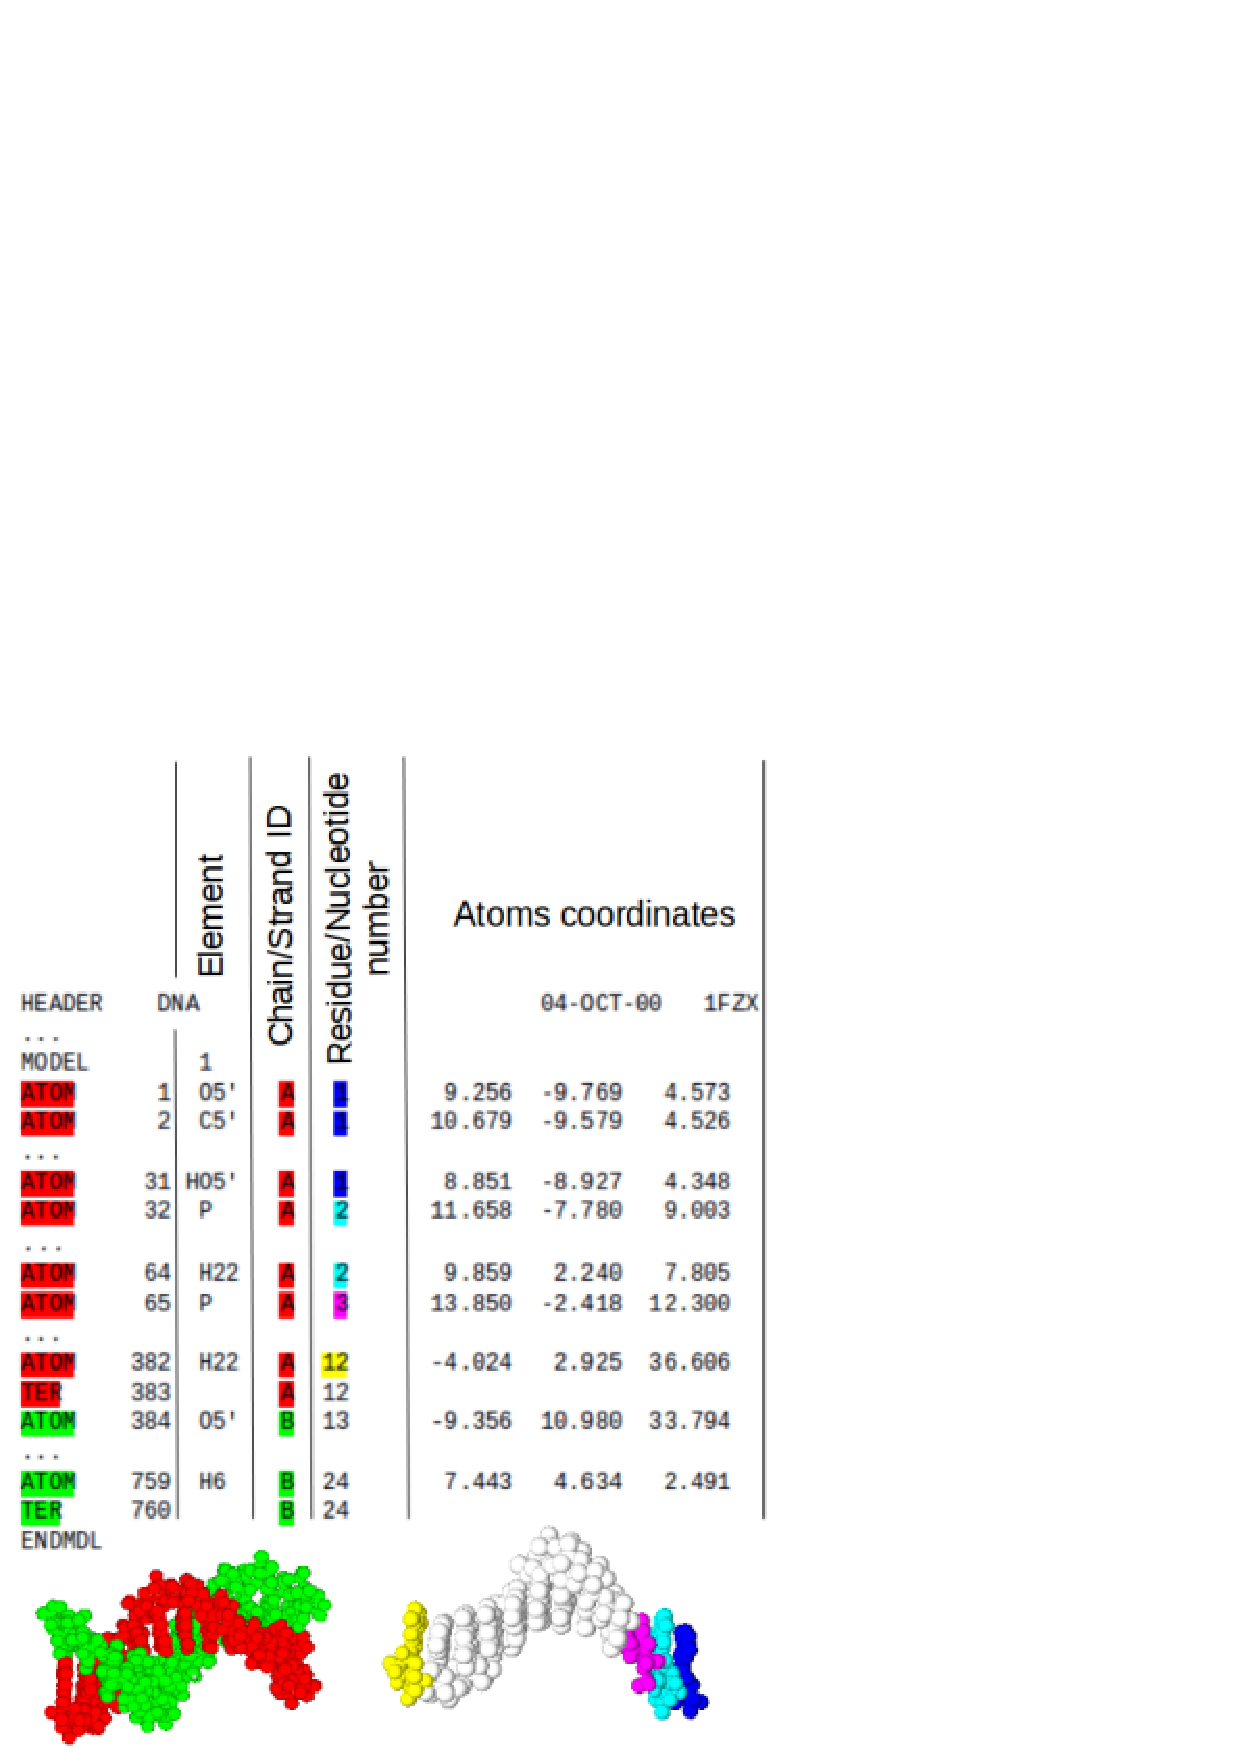
\includegraphics[width=.5\linewidth]{./Figures/pdb.png}
    \caption[Esquema de un PDB]{Esquema de un PDB y molecula vista en vmd(visual molecular dinamics)}
    \label{fig:pdbesq}
\end{figure}

\subsubsection{pdb reader}
Está funcionalidad presente en PDBlib permite leer la estructura molecular de un pdb en Geant4 sin la necesidad de usar otras librerías de terceros, la función se encarga de recolectar la siguiente información: elemento, id de cadena, numero de residuo y coordenadas del átomo, mediante el uso de palabras clave como ATOM y TER\cite{pdblib}.
\subsubsection{Visualización}
Pdb4dna viene preestablecido con la molécula 1ZBB esto debido a que describe la estructura de ADN más grande que se encuentre en formato pdb, el ejemplo hace uso de la geometría de Geant4 simplemente para objetivos de visualización como formas, distribución espacial, materiales y atributos de visualización para cada átomo, por ahora PDB4DNA solo presenta tres modos de visualización, esferas ligadas(baricentros), vista atómica (VDW) y residuos\cite{pdblib}.

\begin{figure}[htbp]
    \centering
    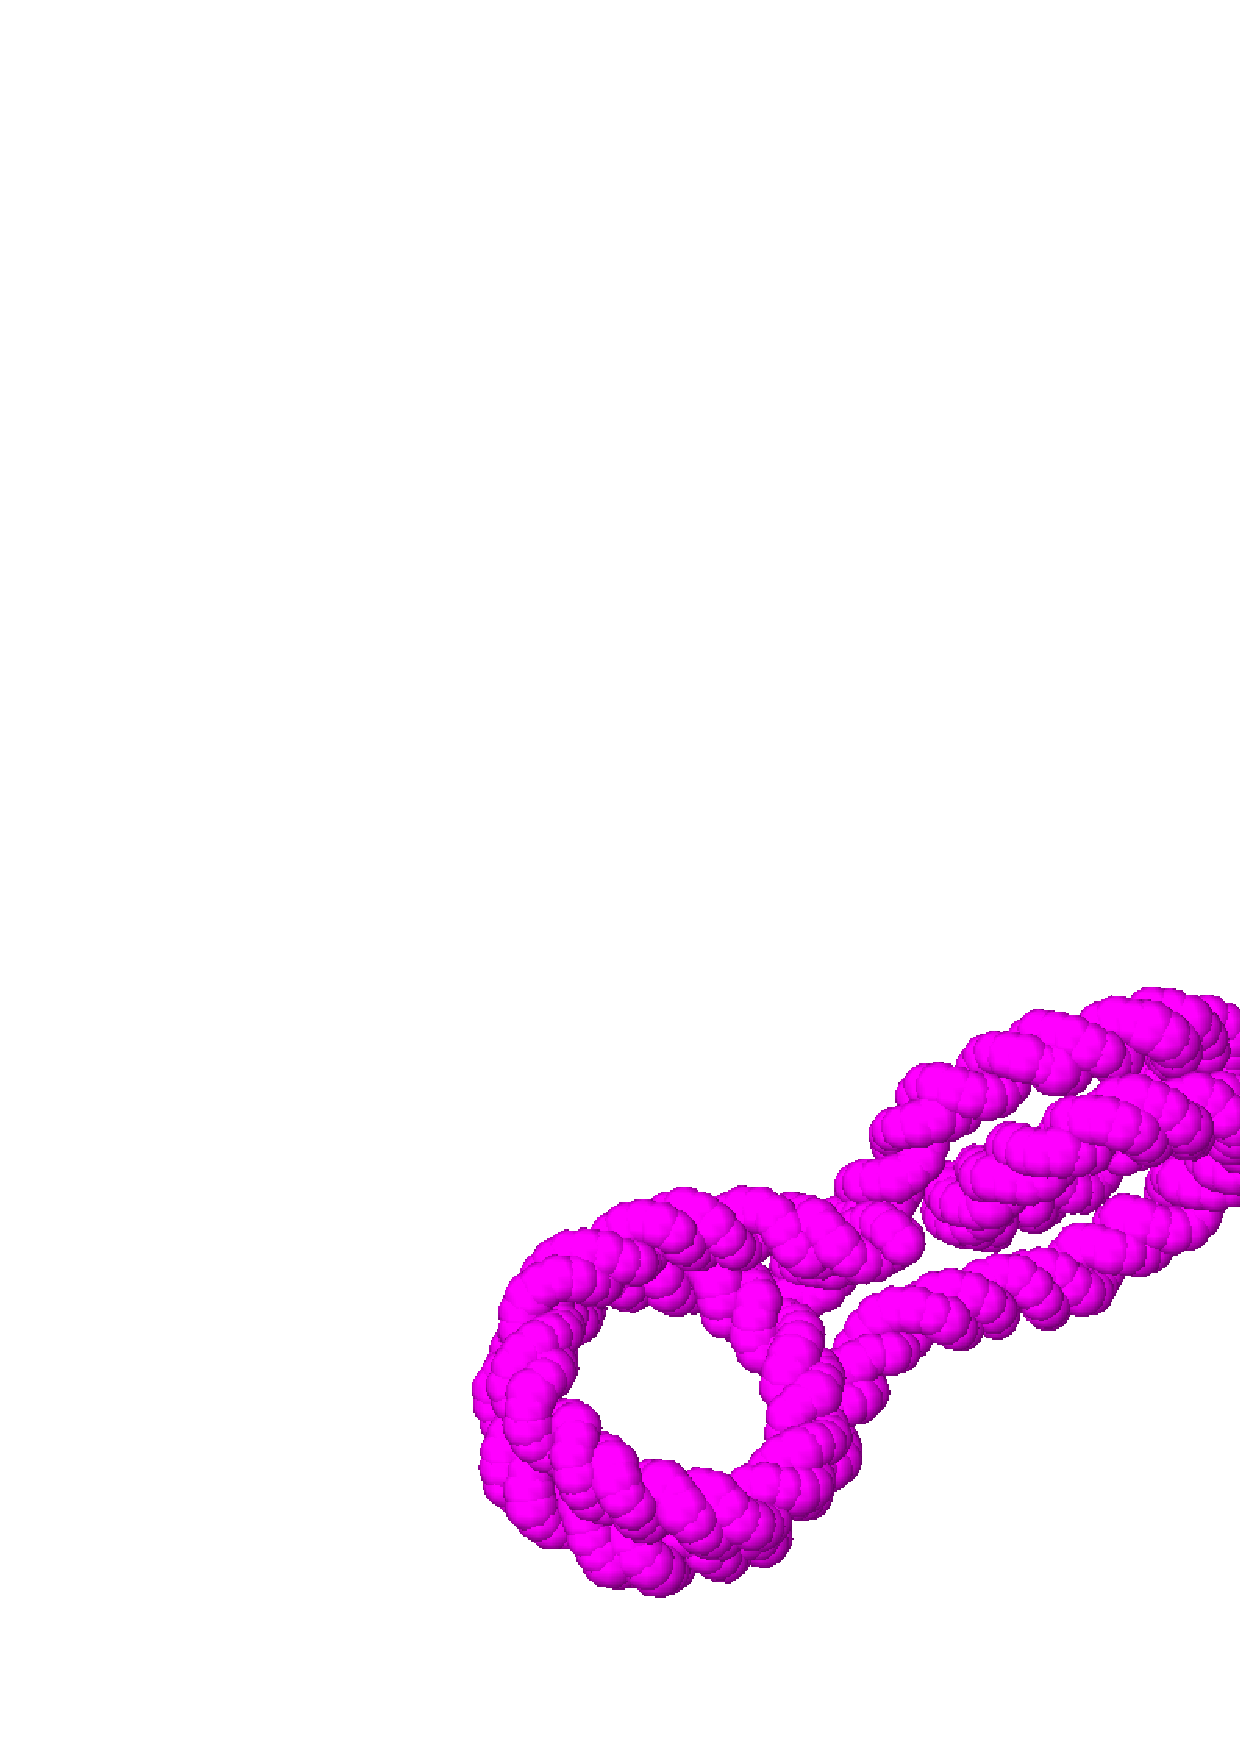
\includegraphics[width=.7\linewidth]{./Figures/ba.png}
    \caption{Barycentros}
    \label{fig:ba}
\end{figure}


\begin{figure}[htbp]
    \centering
    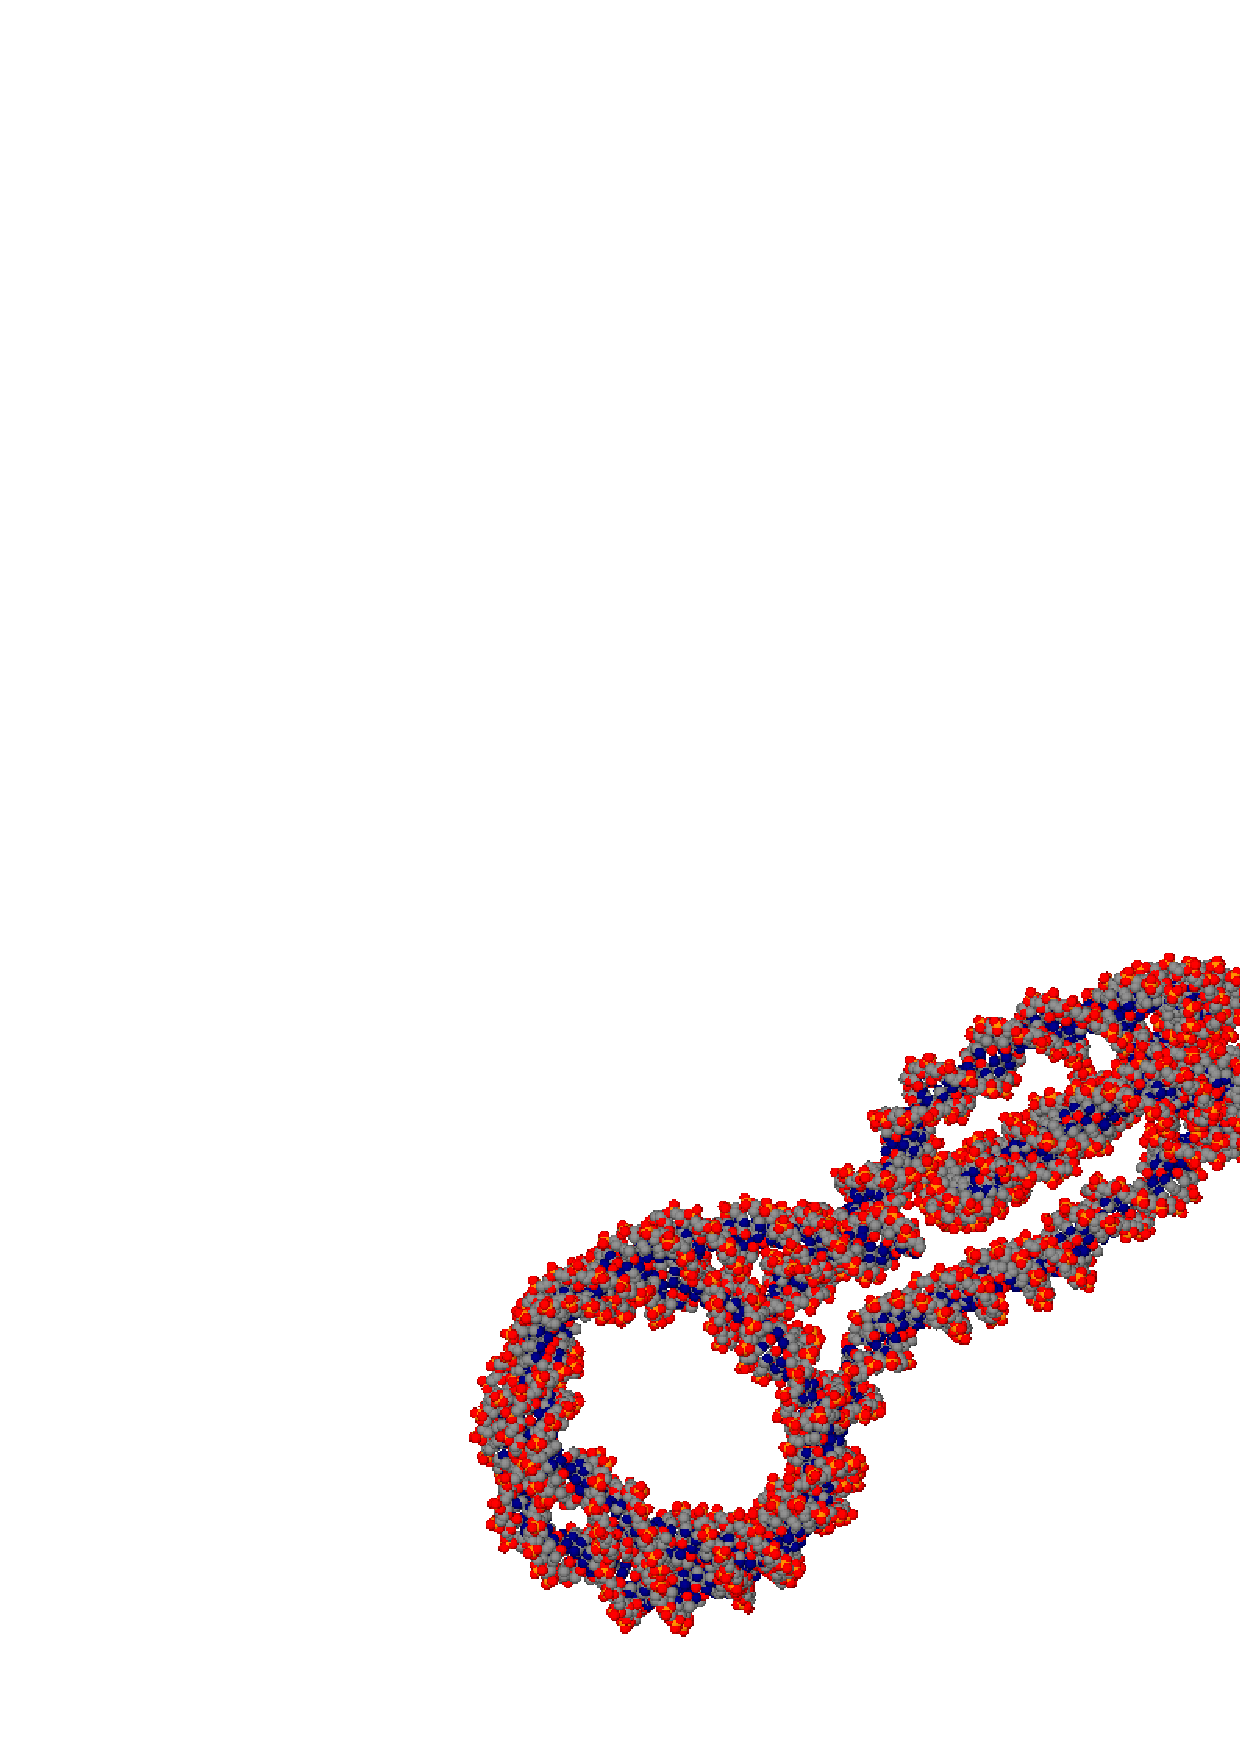
\includegraphics[width=.7\linewidth]{./Figures/cpk.png}
    \caption{VDW}
    \label{fig:cpk}
\end{figure}

\begin{figure}[htbp]
    \centering
    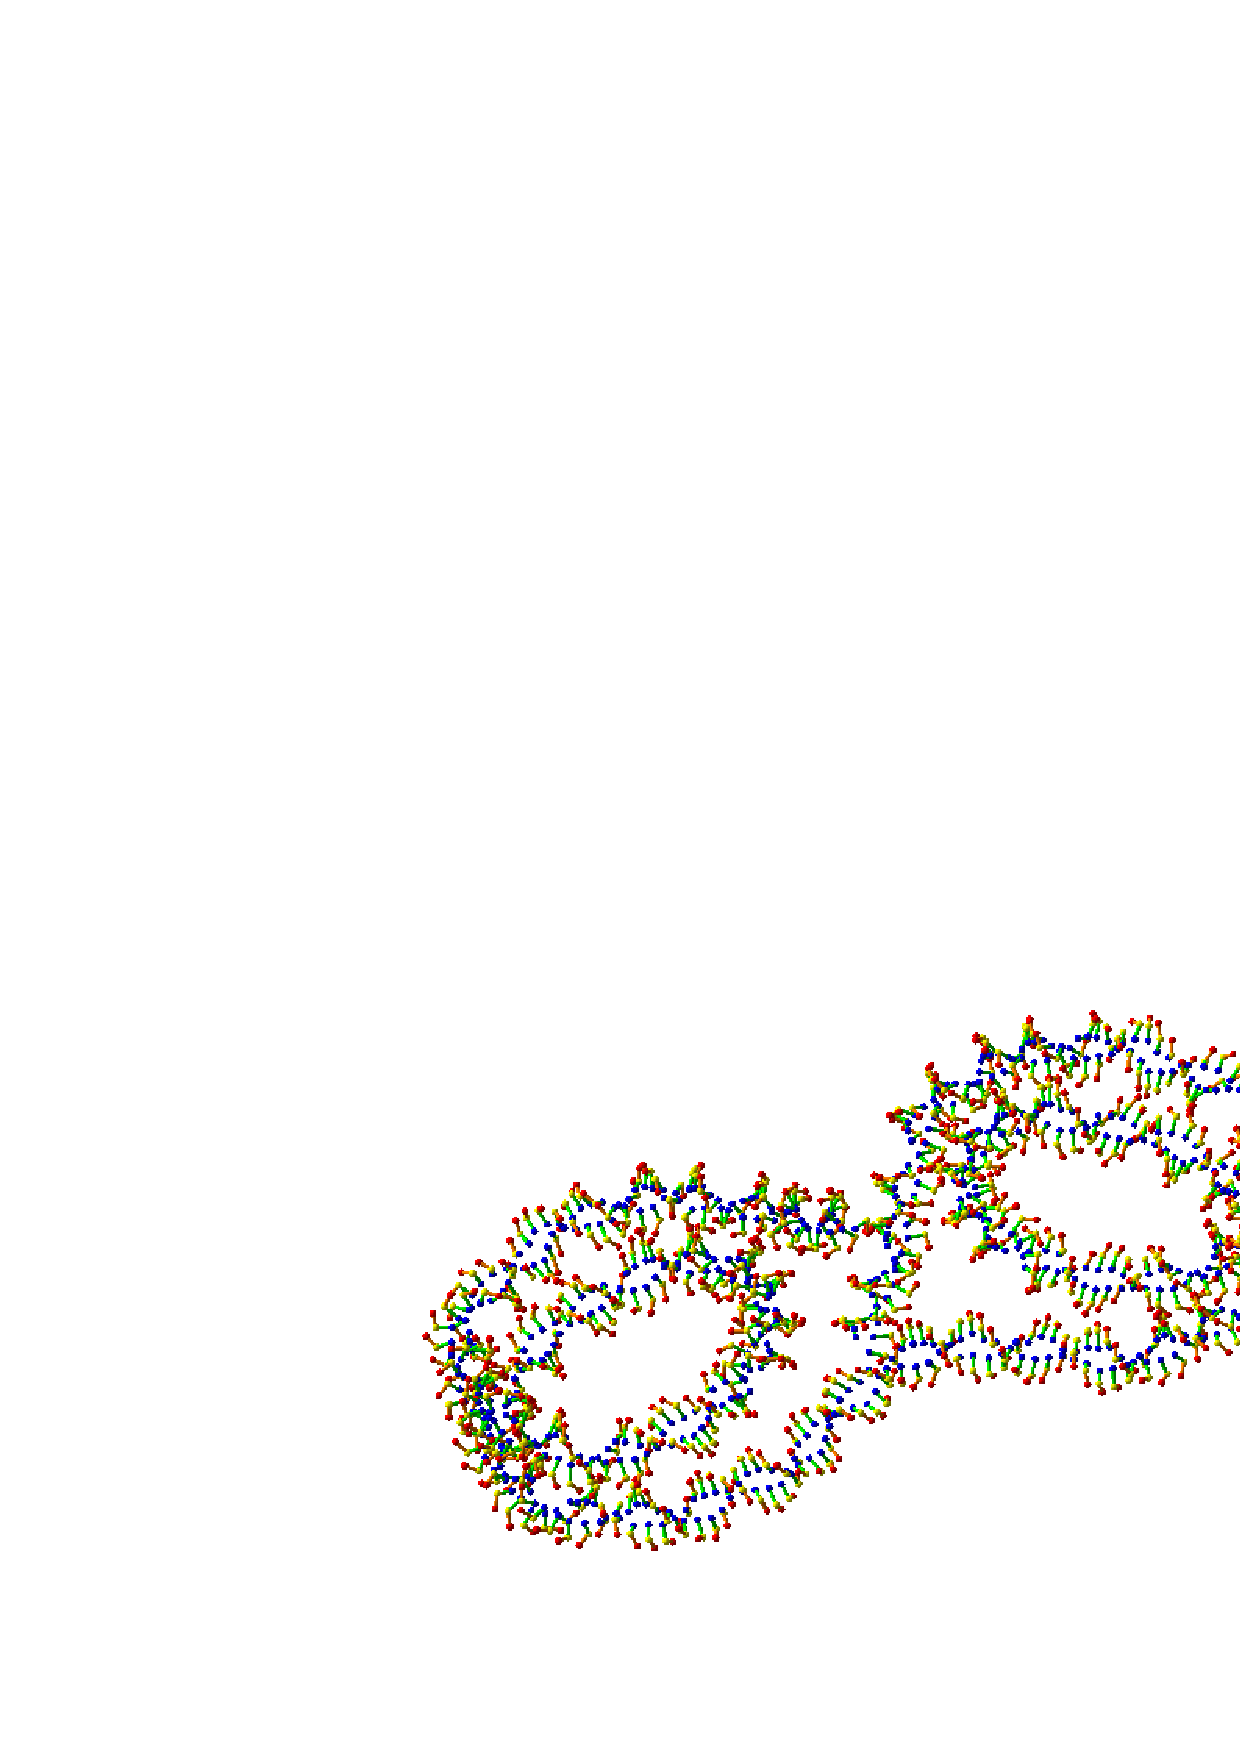
\includegraphics[width=.7\linewidth]{./Figures/re.png}
    \caption{Residuos}
    \label{fig:re}
\end{figure}

\subsubsection{Simulación}
Debido a que Geant4 no contiene secciones transversales definidas para ADN, las simulaciones son realizadas en agua y las deposiciones de energía resultantes son entonces alocadas en grupos de átomos constituyendo la molécula de ADN, para este propósito se hace uso de un bounding box(caja delimitadora) el cual es un volumen constituido de agua con dimensiones correspondientes a la respectiva molécula de ADN, la lista de física empleada es Geant4-DNA adaptada a micro y nano dosimetría, los procesos de esta extienden la física para electrones, hidrógeno, átomos de helio y algunos iones\cite{pdblib}.

\subsubsection{Algoritmo para encontrar el atomo más cercano}
Es necesario el uso de un algoritmo cuyo objetivo de este es alocar la deposición de energía en un elemento(azúcar base o fosfato) del nucleótido para luego deducir rompimientos de cadena simples y rompimientos dobles.
Para empezar se forman múltiples esferas a partir del baricentro geométrico de cada nucleótido, el radio de cada esfera es la máxima distancia entre el baricentro y las coordenadas de los átomos que constituyen el nucleótido, incluyendo el máximo radio de Van der Waals (1.8 Angstrom para el elemento del fósforo), si una deposición de energía es localizada en una esfera ligada un segundo proceso verifica los radios de Van der Waals, para encontrar el átomo del nucleótido más cercano a dicha deposición. debido a que las esferas ligadas de los nucleótidos se superponen , los dos nucleótidos más cercanos son incluidos en el algoritmo, cuando se cumple un evento, el algoritmo retorna la deposición de energía, la cadena de ADN, el id de nucleótido, y el id del grupo sea base, fosfato o azúcar, todo este proceso puede verse con más claridad en las figuras ~\ref{fig:deepbox} y ~\ref{fig:algoritmo}.


\begin{figure}[htbp]
    \centering
    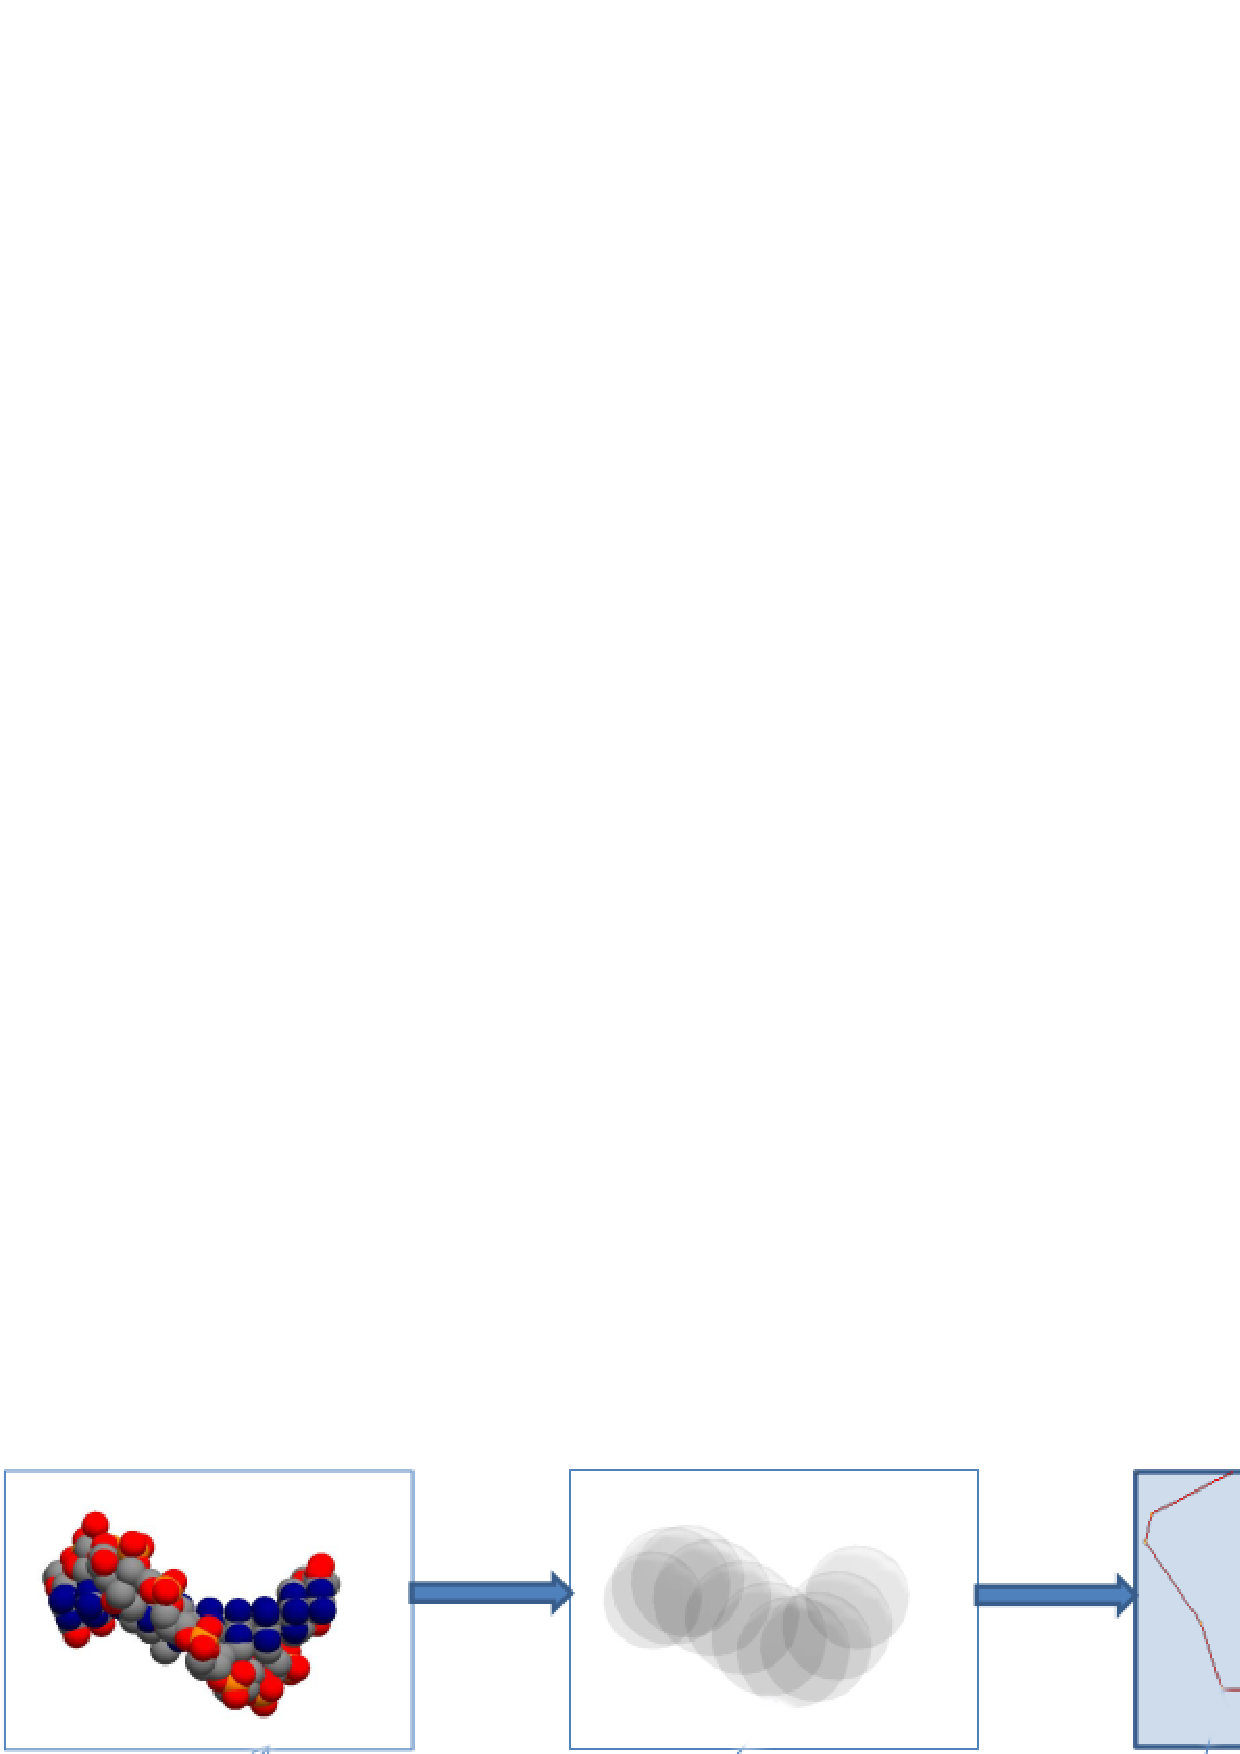
\includegraphics[width=.8\linewidth]{./Figures/aalgo.png}
    \caption[Caja delimitadora]{Caja delimitadora, lista de esferas, deposición de energía, imagen tomadas de \cite{handson} }
    \label{fig:deepbox}
\end{figure}

\begin{figure}[htbp]
    \centering
    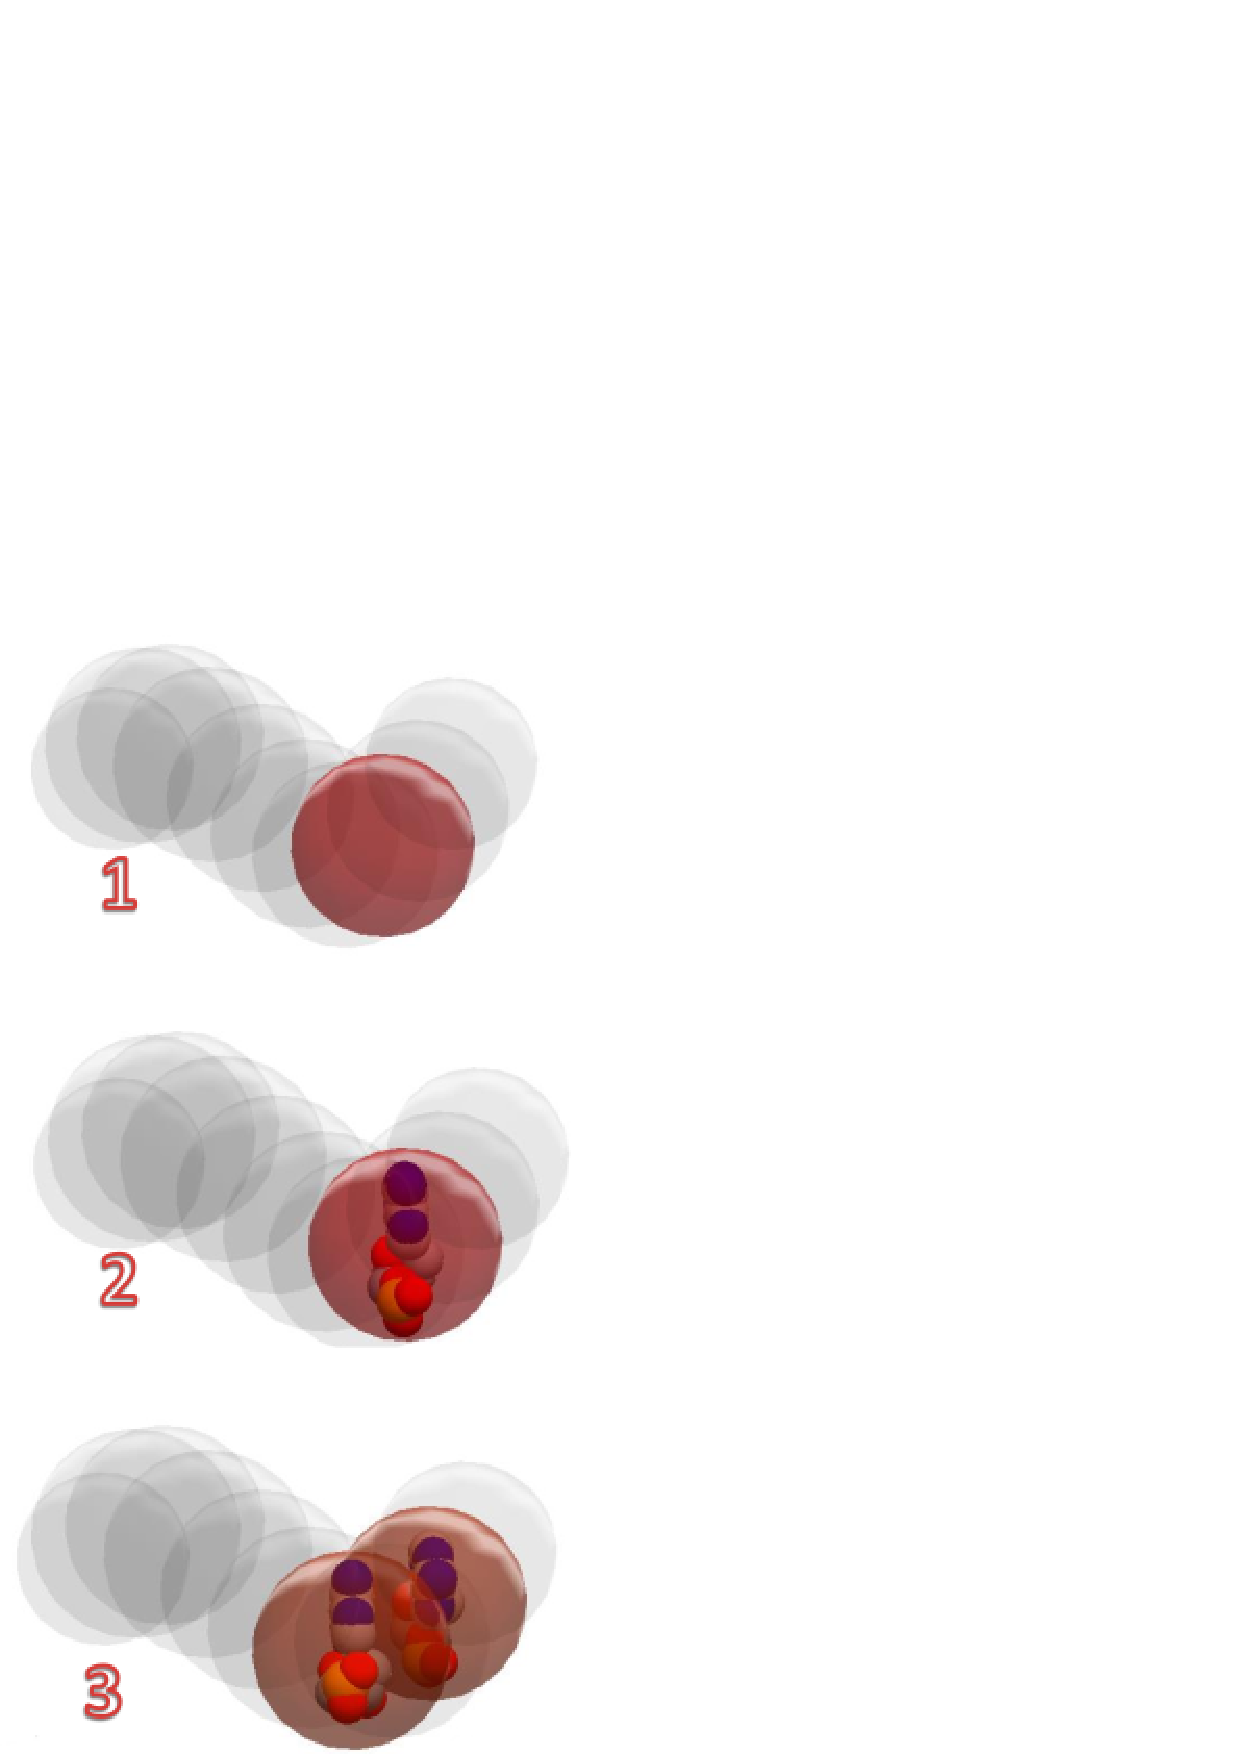
\includegraphics[width=.3\linewidth]{./Figures/algo.png}
    \caption[Esferas ligadas y nucleótidos]{Esferas ligadas y nucleótidos, imagen tomada de \cite{handson}}
    \label{fig:algoritmo}
\end{figure}

\subsubsection{Rompimientos simples y dobles}
El calculo de rompimientos simples se hace a partir  de la asunción de que la energía sobrepase un estimado de 8.22 eV en un grupo de azúcar fosfato, es decir en un enlace fosfodiéster, para los rompimientos dobles se asume que la distancia máxima son diez pares base separando dos rompimientos simples en cadenas de ADN opuestas, cuando esto sucede se considera que ha sucedido un rompimiento doble\cite{pdblib}, esto puede ser observado en la figura ~\ref{fig:sbdb}.

\begin{figure}[htbp]
    \centering
    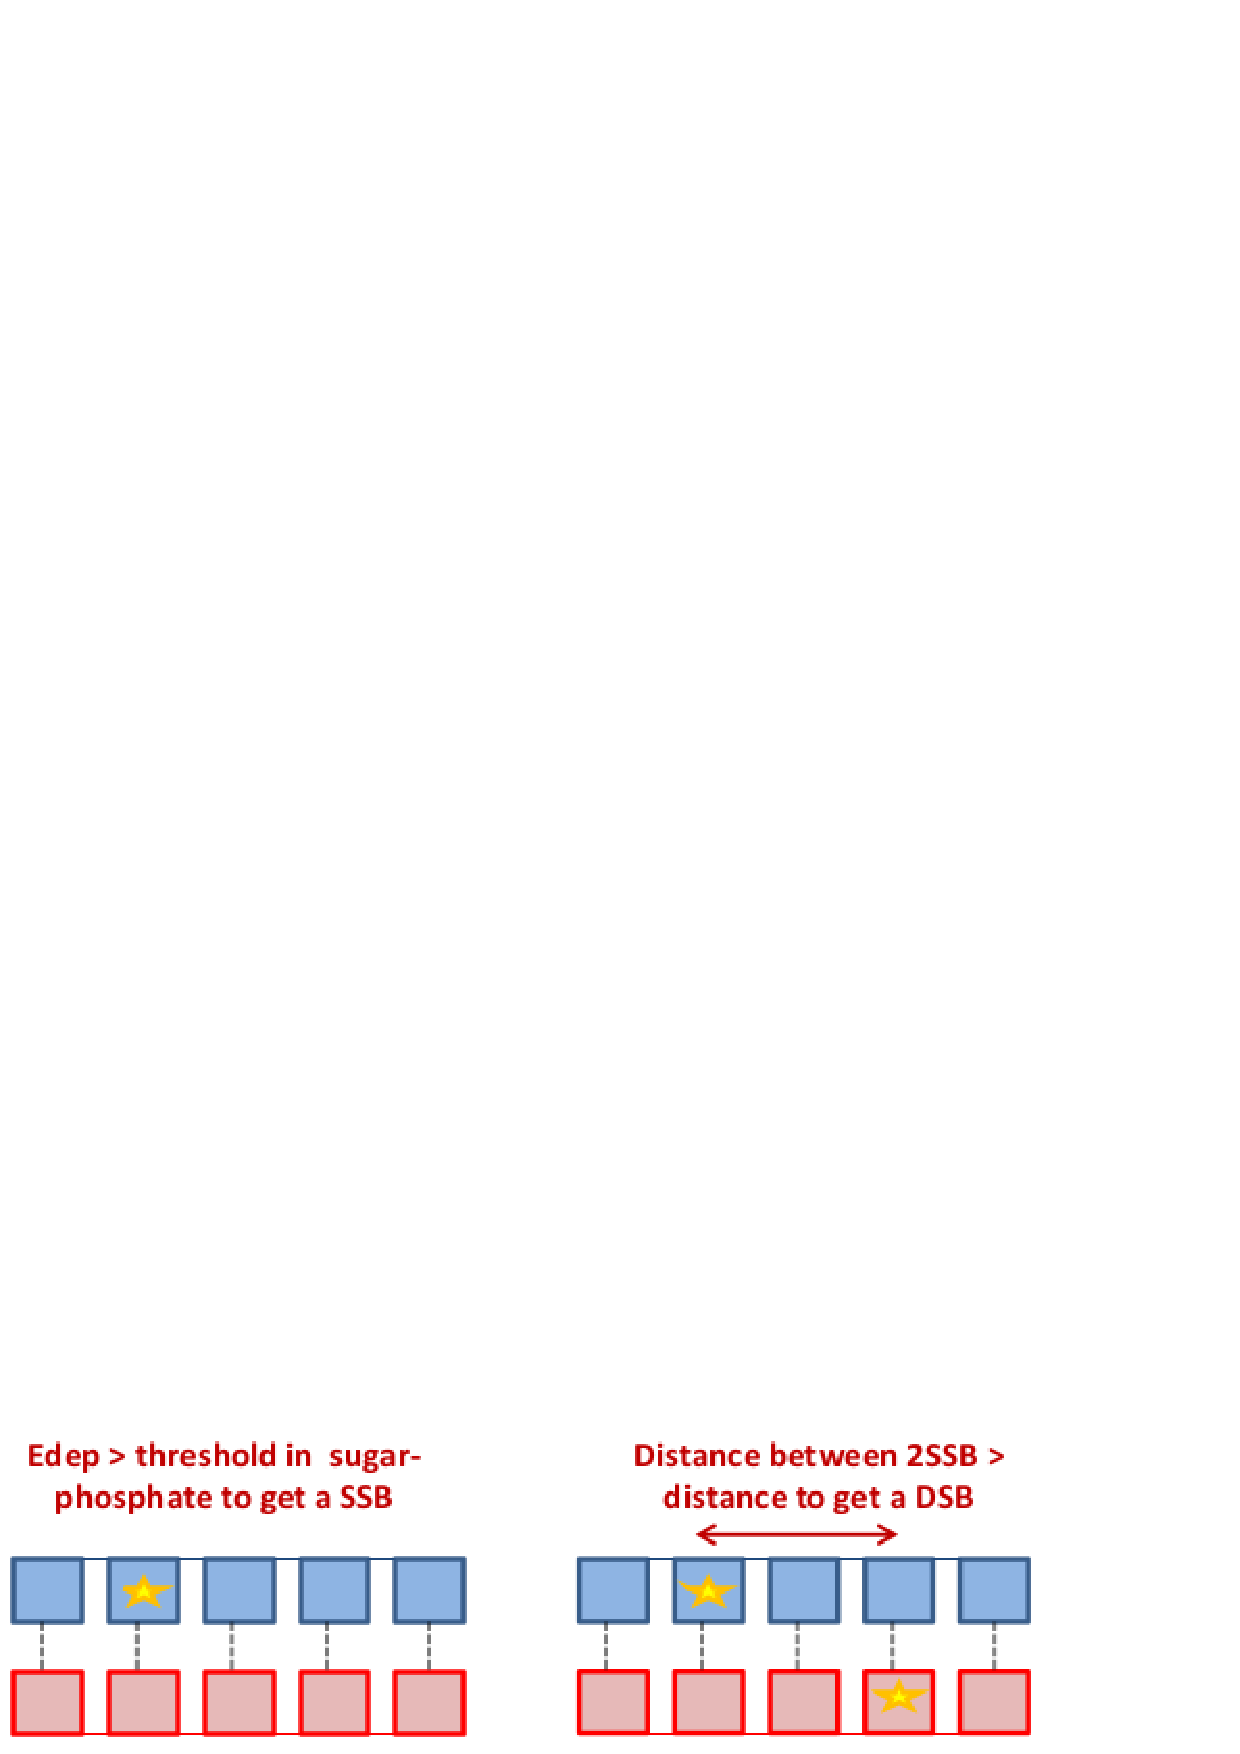
\includegraphics[width=.8\linewidth]{./Figures/romp.png}
    \caption[Esquema rompimientos simples y dobles en el ADN]{Esquema rompimientos simples y dobles en el ADN, imagen tomada de \cite{handson} }
    \label{fig:sbdb}
\end{figure}

Al principio de la simulación se crea un registro para cada cadena de ADN, los valores de dicho registro corresponden a los id de los nucleótidos y la deposición total de energía por cada evento, lo cual se tiene correlación al seguimiento de una partícula primaria y todas sus  segundarías, los registros son actualizados cada vez que el algoritmo para encontrar el átomo más cercano se completa correctamente, al final de cada evento, los registros son leídos para computar el numero de rompimientos simples y dobles, cuando la simulación termina se almacena  en un histograma de ROOT la energía total de deposición en la caja de agua,y el numero de rompimientos simples y dobles\cite{pdblib}, como muestra la figura ~\ref{fig:histosbdb}.

\begin{figure}[htbp]
    \centering
    \includegraphics[width=1\linewidth]{./Figures/c1.png}
    \caption[Histograma de Root]{Histograma de Root y visualización en Geant4}
    \label{fig:histosbdb}
\end{figure}

\subsubsection{Archivos Relevantes}
Todos los ejemplos de Geant4 se componen de múltiples archivos cada uno con un propósito, esta sección aborda una explicación de los archivos fundamentales para entender pdb4dna. Un diagrama de flujo con todos los archivos de pdb4dna puede ser visto en la figura ~\ref{fig:UoC}.

\paragraph{PhysicsList}
Se encarga de llamar la física relevante para cada ejemplo, en este caso se trata de la librería "G4EmDNAPhysics" la cual contiene diversos fenómenos y procesos adaptados para nano y micro dosimetria, algunos de estos fenómenos son dispersión de Compton, dispersión de Rayleigh, efecto fotoeléctrico, etc.

\begin{figure}[htbp]
    \centering
    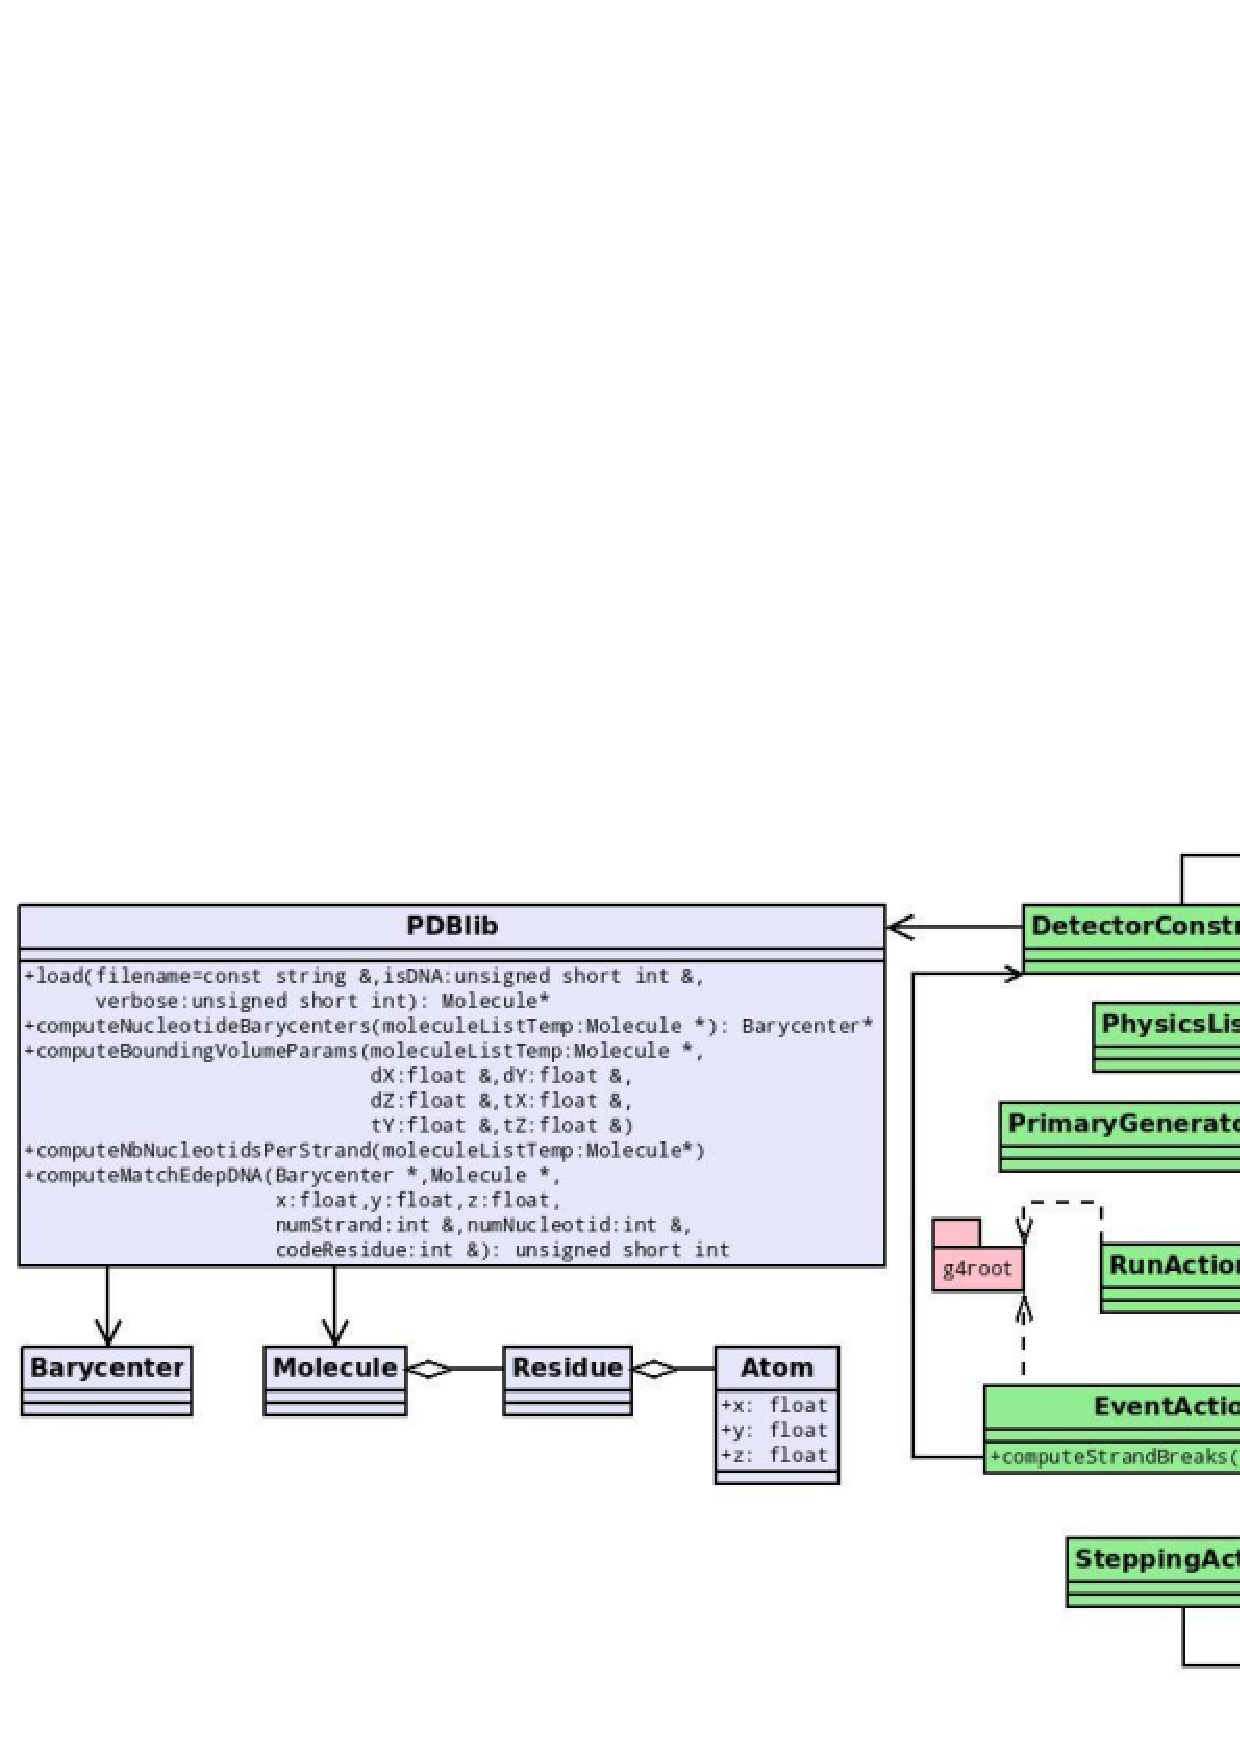
\includegraphics[width=1\linewidth]{./Figures/flujo.png}
    \caption[Diagrama de flujo de PDB4DNA]{Diagrama de flujo de PDB4DNA:Geant4 user application: Clases virtuales Geant4  (blanco), clases implementadas Geant4 (verde), libreria PDB (morado) y interfaz para análisis en Root (rojo), imagen tomada de \cite{pdblib}.}
    \label{fig:UoC}
\end{figure}

\paragraph{PDBlib}

PDBlib es básicamente el corazón de PDB4DNA, es el encargado de leer el archivo de pdb, identificar si este es ADN, luego identifica las diferentes partes de la molécula de ADN como es la base, el fosfato, y el azúcar, y como el resto del código puede identifica estos para llevar a cabo el calculo de rompimientos simples y dobles, ademas de ello se encarga de crear los diferentes tipos de visualización los cuales son exportados a DetectorConstruction, contiene el algoritmo para encontrar el átomo más cercano a la deposición de energía ya mencionado anteriormente.



\paragraph{DetectorConstruction}
En Geant4 este archivo se encarga de crear y posicionar los diferentes volúmenes que sean relevantes para la simulación, en el ejemplo pdb4dna es algo curioso que DetectorConstruction funciona como un archivo más de visualización para crear diferentes representaciones de la molécula de ADN, tal como se observa en las figuras: ~\ref{fig:ba}, ~\ref{fig:cpk}, ~\ref{fig:re}, sin embargo es pertinente mencionar que igual mantiene su objetivo de controlar características relevantes para la simulación como el tamaño del mundo( volumen madre donde se encuentran otros volúmenes) y el bounding box ya mencionado anteriormente.


\paragraph{SteppingAction}
Es el encargado de seguir la deposición de energía en el bounding box, primero el PDBlib se encarga de asignar un numero en base a la estructura del ADN es decir se asignan los valores numéricos: 0 para el fosfato, 1 para el azúcar y 2 para la base, esto se realiza mediante la estructura del pdb, cuando se corre un evento SteppingAction se encarga de calcular la deposición de energía en cada uno de estos, debido a que es un enlace fosfodiester el programa solo retorna los valores de energía depositados en el fosfato o el azúcar, estos valores son enviados a subsecuentes librerías las cuales se encargan de realizar un conteo que consiste en que si la energía sobrepasa el valor de 8.22 eV cuenta como un rompimiento simple y si en 10 pares base en la cadena opuesta se presenta otro rompimiento se toma como rompimiento doble, como se muestra en la figura ~\ref{fig:sbdb}, luego todos estos datos para múltiples eventos son enviados a un archivo Root para la visualización del histograma.


% SEC5

\clearpage

\section{Modificaciones PDB4DNA}
\label{sec:MODIFI}
PDB4DNA fue modificado de tal manera que en vez de hacer uso de las esferas ligadas a partir de barycentros usara centros de masa, para esto se uso el archivo PDBlib, primero se definió la masa de los diferentes elementos (véase anexo ~\ref{app:A}),y luego se usaron las clases bases ya definidas en PDBlib para hacer los respectivos cálculos de centros de masa(véase anexo ~\ref{app:B}).\\


% SEC6
\clearpage
\section{Conclusiones}
\label{sec:res}
Se ha mostrado que pdb4dna es una aplicación bastante interesante de Geant4 la cual permite realizar cálculos de deposición de energía y conteos tanto de rompimientos simples como dobles de ciertas moléculas de ADN mediante un archivo pdb con ciertas condiciones, bien la aplicación puede ser extendida al uso de moléculas de ADN más complejas y también otros tipos de moléculas, a partir de la energía depositada se presenta la posibilidad de modificar el código de manera que sabiendo donde se deposita la energía y el filtro poder realizar una localización de los rompimientos simples y dobles en la molécula de ADN lo cual permitiría el uso de gromacs para estudiar la dinámica propia de está.\\
En otra instancia también se modifico Geant4 para que usara centros de masa en lugar de esferas ligadas basadas en baricentros, al realizar histogramas tanto de las esferas ligadas y los baricentros no se ve ninguna diferencia en la deposición de energía ni en los rompimientos simples como dobles bajo las mismas condiciones de eventos, partículas, y energía. Esto se podría deber a que el código no esta tomando correctamente los centros de masa nuevos o a que el valor de la magnitud de las masas no afecta de forma relevante las posiciones del centro de masa respecto a las de los baricentros, sin embargo de ser la segunda opción esto podría cambiar de forma relevante con moléculas mucho más complejas o grandes debido a que como se observo en los histogramas de las diferentes posiciones de centros de masa contra baricentros se observan cambios a simple vista en las posiciones lo que resultaría en un cambio de la deposición de energía y en consecuencia de los rompimientos y posterior dinámica estructural, lo anterior se hizo con el fin de proponer un modelo alterno diferente a las esferas ligadas en baricentros con el fin de que sea más acercado al modelo general de átomos y masa.


% SEC7
%\input{./Sections/Seccion_7}



%%%%%%%%%%%%%%%%%%%%%%%%%%%%%%%%%%%%%%%%%%%%%%%%%%%%%%%%%%%%%
%APPENDICES
%%%%%%%%%%%%%%%%%%%%%%%%%%%%%%%%%%%%%%%%%%%%%%%%%%%%%%%%%%%%%


\appendix
\renewcommand*{\thesection}{\Alph{section}}\textbf{}

% APPENDIX A
\clearpage
\section{Anexo}
\label{app:A}
\lstset {language=C++}
\begin{lstlisting}
      double TotalMass = 0.0;
      double TotalMassPhosResSeq1 = 0.0;
      double TotalMassSugResSeq1 = 0.0;
      double TotalMassBaseResSeq1 = 0.0;
      double TotalMassPhosResSeq2 = 0.0;
      double TotalMassSugResSeq2 = 0.0;
      double TotalMassBaseResSeq2 = 0.0;


      for(int i = 0; i < residueListTemp->fNbAtom; i++)
      {
	//EM
      	//////////////////////////////////////
	// Set Mass expressed in u
        double ElementMass = 0.0;
        if(AtomTemp->fElement == "H") ElementMass = 1.00784;
	else if(AtomTemp->fElement == "C") ElementMass = 12.0107;
        else if(AtomTemp->fElement == "N") ElementMass = 14.0067;
        else if(AtomTemp->fElement == "O") ElementMass = 15.999;
        else if(AtomTemp->fElement == "P") ElementMass = 30.973762;
        else if(AtomTemp->fElement == "S") ElementMass = 32.065;
        else
	  {
          G4cerr << "Element not recognized : " << AtomTemp->fElement << G4endl;
          G4cerr << "Stop now" << G4endl;
          exit(1);
        }
\end{lstlisting}
\section{Anexo}
\label{app:B}
\lstset {language=C++}
\begin{lstlisting}
//Center of mass calculation
else if( OptCalc == 2 )
  {
    baryX += ElementMass * (AtomTemp->fX);
    baryY += ElementMass * (AtomTemp->fY);
    baryZ += ElementMass * (AtomTemp->fZ);
    TotalMass += ElementMass;

    if(residueListTemp->fResSeq == 1)
      {
  if(i == 0)
    {
      baryPhosX += ElementMass * (AtomTemp->fX);
      baryPhosY += ElementMass * (AtomTemp->fY);
      baryPhosZ += ElementMass * (AtomTemp->fZ);
      TotalMassPhosResSeq1 += ElementMass;
    }
  else if(i < 8)
    {
      barySugX += ElementMass * (AtomTemp->fX);
      barySugY += ElementMass * (AtomTemp->fY);
      barySugZ += ElementMass * (AtomTemp->fZ);
      TotalMassSugResSeq1 += ElementMass;
    }
  else
    {
      //hydrogen are placed at the end of the residue in a PDB file
      //We don't want them for this calculation
      if(AtomTemp->fElement != "H")
        {
    baryBaseX += ElementMass * (AtomTemp->fX);
    baryBaseY += ElementMass * (AtomTemp->fY);
    baryBaseZ += ElementMass * (AtomTemp->fZ);
    TotalMassBaseResSeq1 += ElementMass;
        }
    }
      } //// if(residueListTemp->fResSeq == 1)........
    else  //if(residueListTemp->fResSeq != 1)
      {
  if(i < 4)
    {
      baryPhosX += ElementMass * (AtomTemp->fX);
      baryPhosY += ElementMass * (AtomTemp->fY);
      baryPhosZ += ElementMass * (AtomTemp->fZ);
      TotalMassPhosResSeq2 += ElementMass;
    }
  else if(i < 11)
    {
      barySugX += ElementMass * (AtomTemp->fX);
      barySugY += ElementMass * (AtomTemp->fY);
      barySugZ += ElementMass * (AtomTemp->fZ);
      TotalMassSugResSeq2 += ElementMass;
    }
  else
    {
      //hydrogen are placed at the end of the residue in a PDB file
      //We don't want them for this calculation
      if(AtomTemp->fElement != "H")
        { // break;
    baryBaseX += ElementMass * (AtomTemp->fX);
    baryBaseY += ElementMass * (AtomTemp->fY);
    baryBaseZ += ElementMass * (AtomTemp->fZ);
    TotalMassBaseResSeq2 += ElementMass;
        }
    }

      } // //if(residueListTemp->fResSeq != 1).......
  } //else if( OptCalc == 2 ).....
//Neither OpcCalc=1 nor OptCalc=2
else
  G4cerr << "Something is fishy!! : "  << G4endl;

AtomTemp = AtomTemp->GetNext();
    } //end of for (  i=0 ; i < residueListTemp->nbAtom ; i++)

\end{lstlisting}






%%%%%%%%%%%%%%%%%%%%%%%%%%%%%%%%%%%%%%%%%%%%%%%%%%%%%%%%%%%%%
%BIBLIOGRAPHY
%%%%%%%%%%%%%%%%%%%%%%%%%%%%%%%%%%%%%%%%%%%%%%%%%%%%%%%%%%%%%

\clearpage
\renewcommand*{\thesection}{}\textbf{}

%\bibliographystyle{apacite}
%\bibliography{Bibliography.bib}

\bibliography{Bibliography}

\end{document}
